\mychapter{평면좌표}{}
\section{좌표평면}
\begin{center}
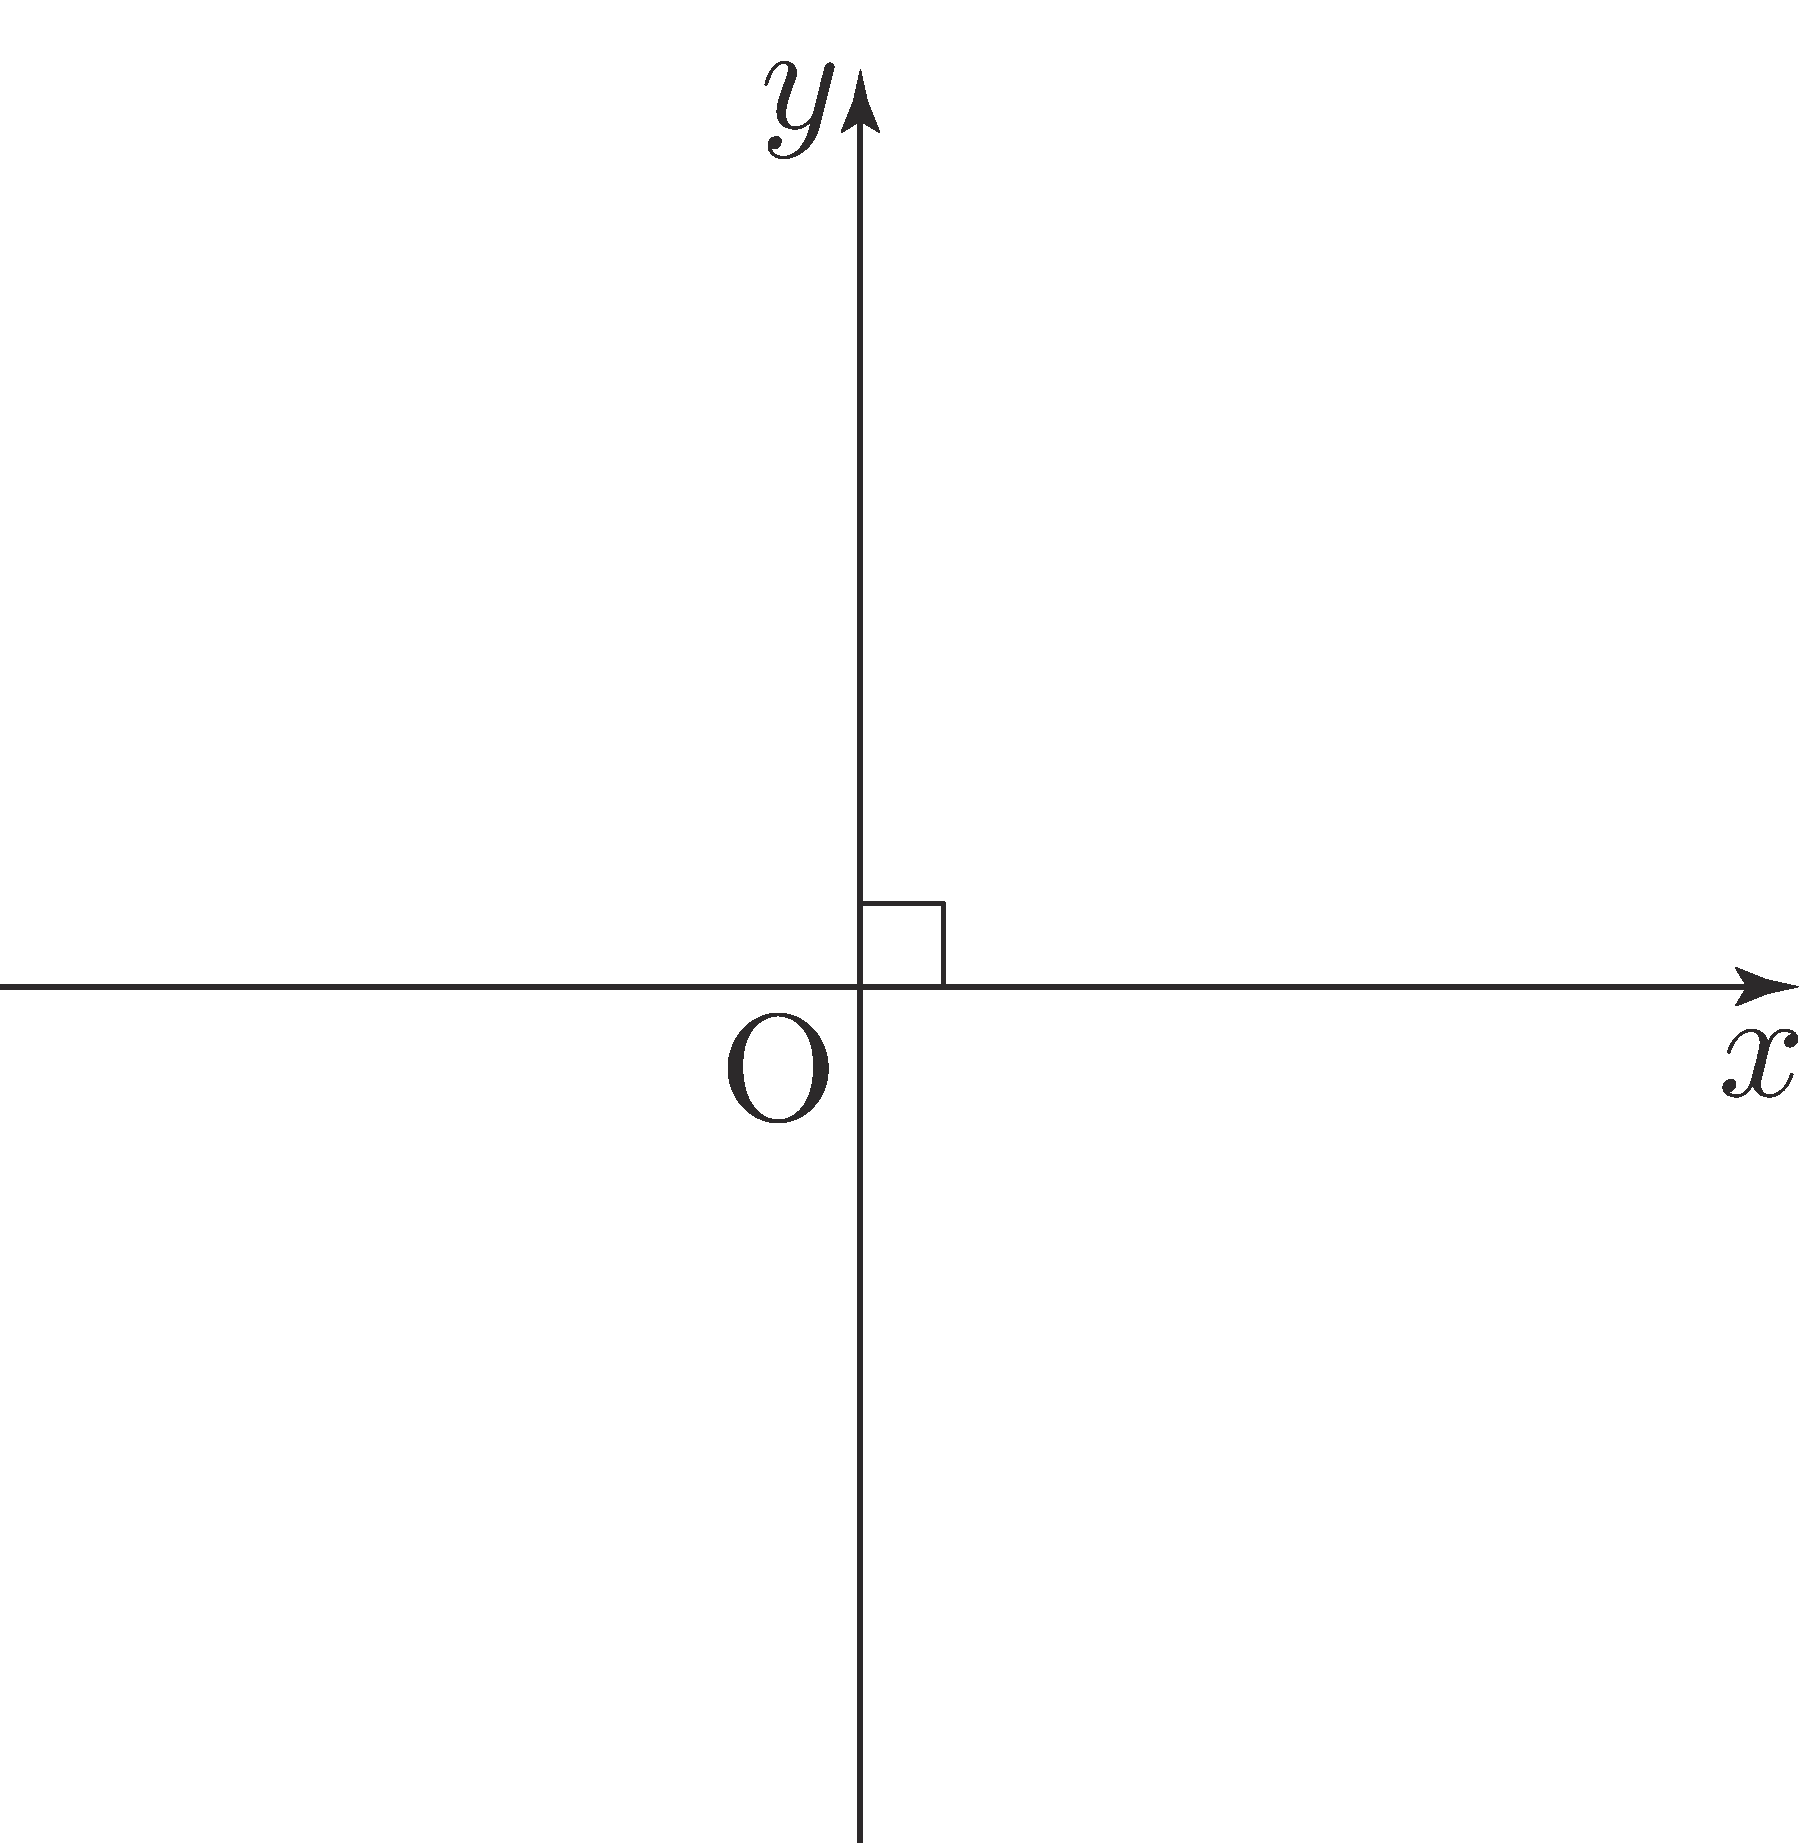
\includegraphics[scale=0.125]{pic0/pic142.pdf}
\end{center}평면의 한 점 $\mrm{O}$에서 서로 직교하는 두 수직선을 그어 각각 $x$축, $y$축이라 하고, 이들을 통틀어 \term[좌표축]{좌표평면에서의 좌표축}{1}이라고 합니다. 이때 점 $\mrm{O}$를 \term[원점]{좌표평면}{1}이라고 합니다. 이와 같이 좌표축이 정해진 평면을 \term{좌표평면}{}이라고 합니다.
\section{평면좌표}
\begin{center}
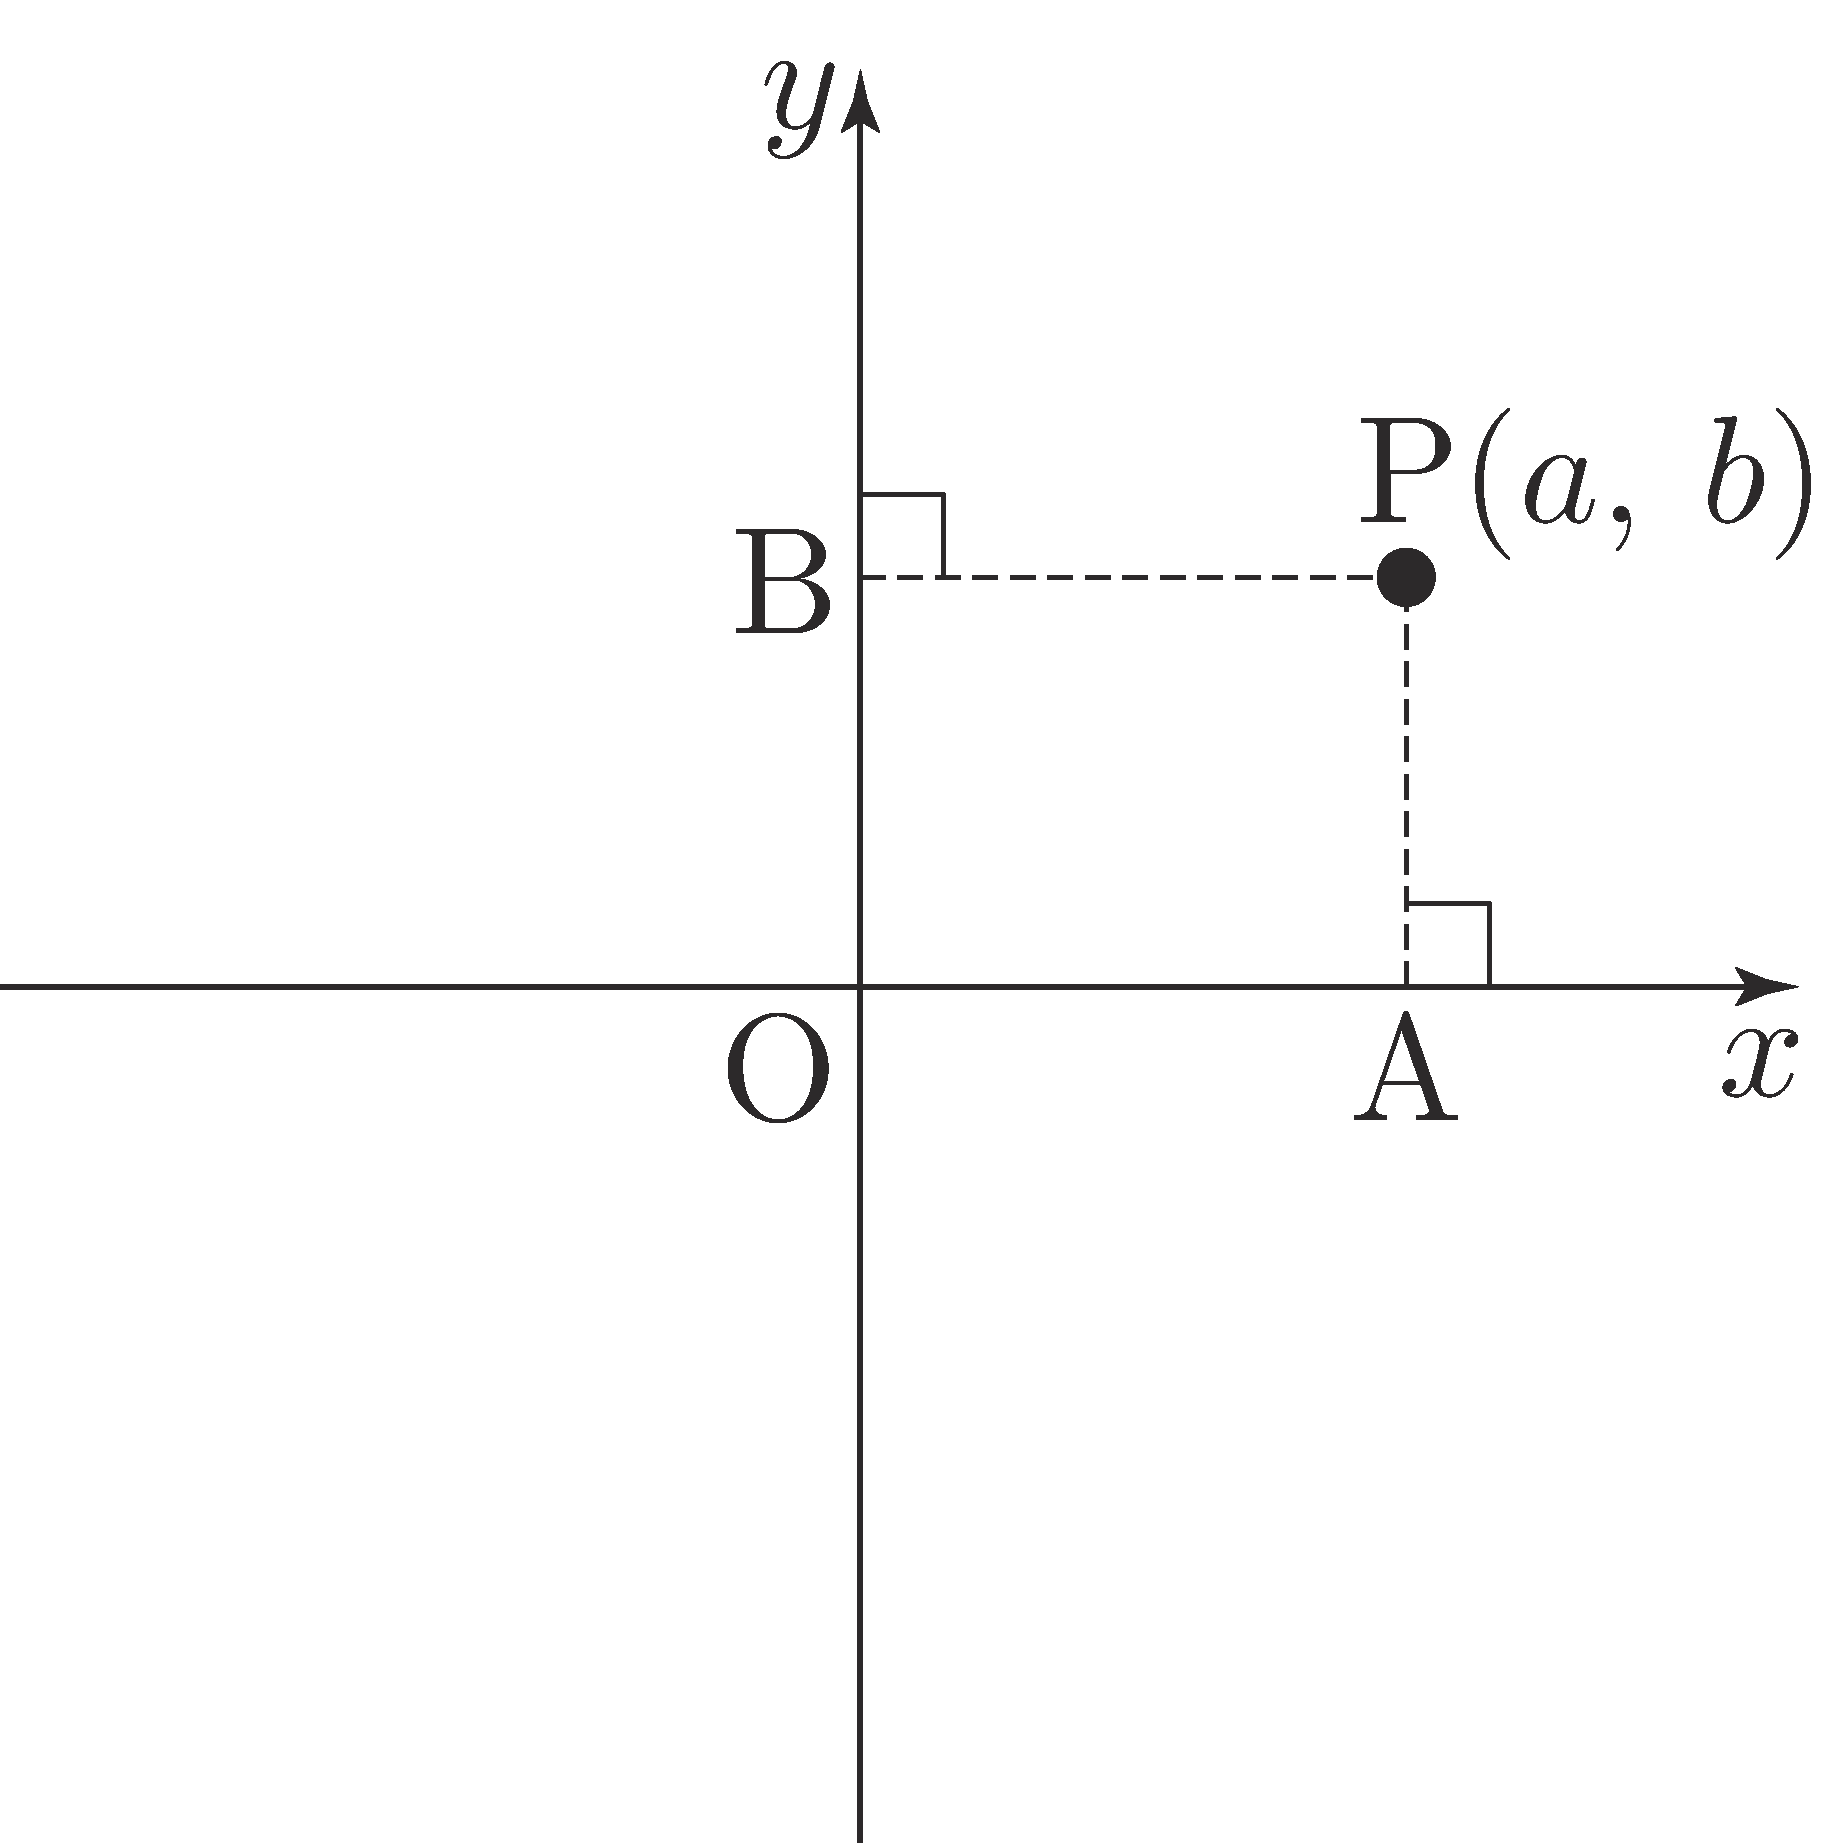
\includegraphics[scale=0.125]{pic0/pic143.pdf}
\end{center}좌표평면의 한 점 $\mrm{P}$에 대하여 점 $\mrm{P}$를 지나고 $x$축, $y$축에 각각 수직인 직선이 이들 축과 만나는 점을 차례로 $\mrm{A}$, $\mrm{B}$라고 하겠습니다. 이때 두 점 $\mrm{A}$, $\mrm{B}$의 $x$축, \mbox{$y$축} 위에서의 좌표를 각각 $a$, $b$라 하면
점 $\mrm{P}$에 대응하는 두 실수의 순서쌍 $\xy{a}{b}$가 정해집니다. 반대로 두 실수의 순서쌍 $\xy{a}{b}$가 주어지면 평면에 있는 한 점 $\mrm{P}$를 대응시킬 수 있습니다.

따라서 평면의 점 $\mrm{P}$와 두 실수의 순서쌍 $\xy{a}{b}$는 일대일로 대응되므로 점 $\mrm{P}$에 대응하는 이 순서쌍을 점 $\mrm{P}$의 \term{평면좌표}{}라 하고, $a$, $b$를 각각 점 $\mrm{P}$의 \term{$x$좌표}{}, \term{$y$좌표}{}라 합니다. 또한 점 $\mrm{P}$의 좌표가 $\xy{a}{b}$일 때 $\xy[P]{a}{b}$라 표기합니다.

\cleartorecto

\term[거리!좌표평면]{두 점 사이의 거리}{0}
\section{두 점 사이의 거리}
{\color{white}.}\\[-1.55\blskip]\begin{center}
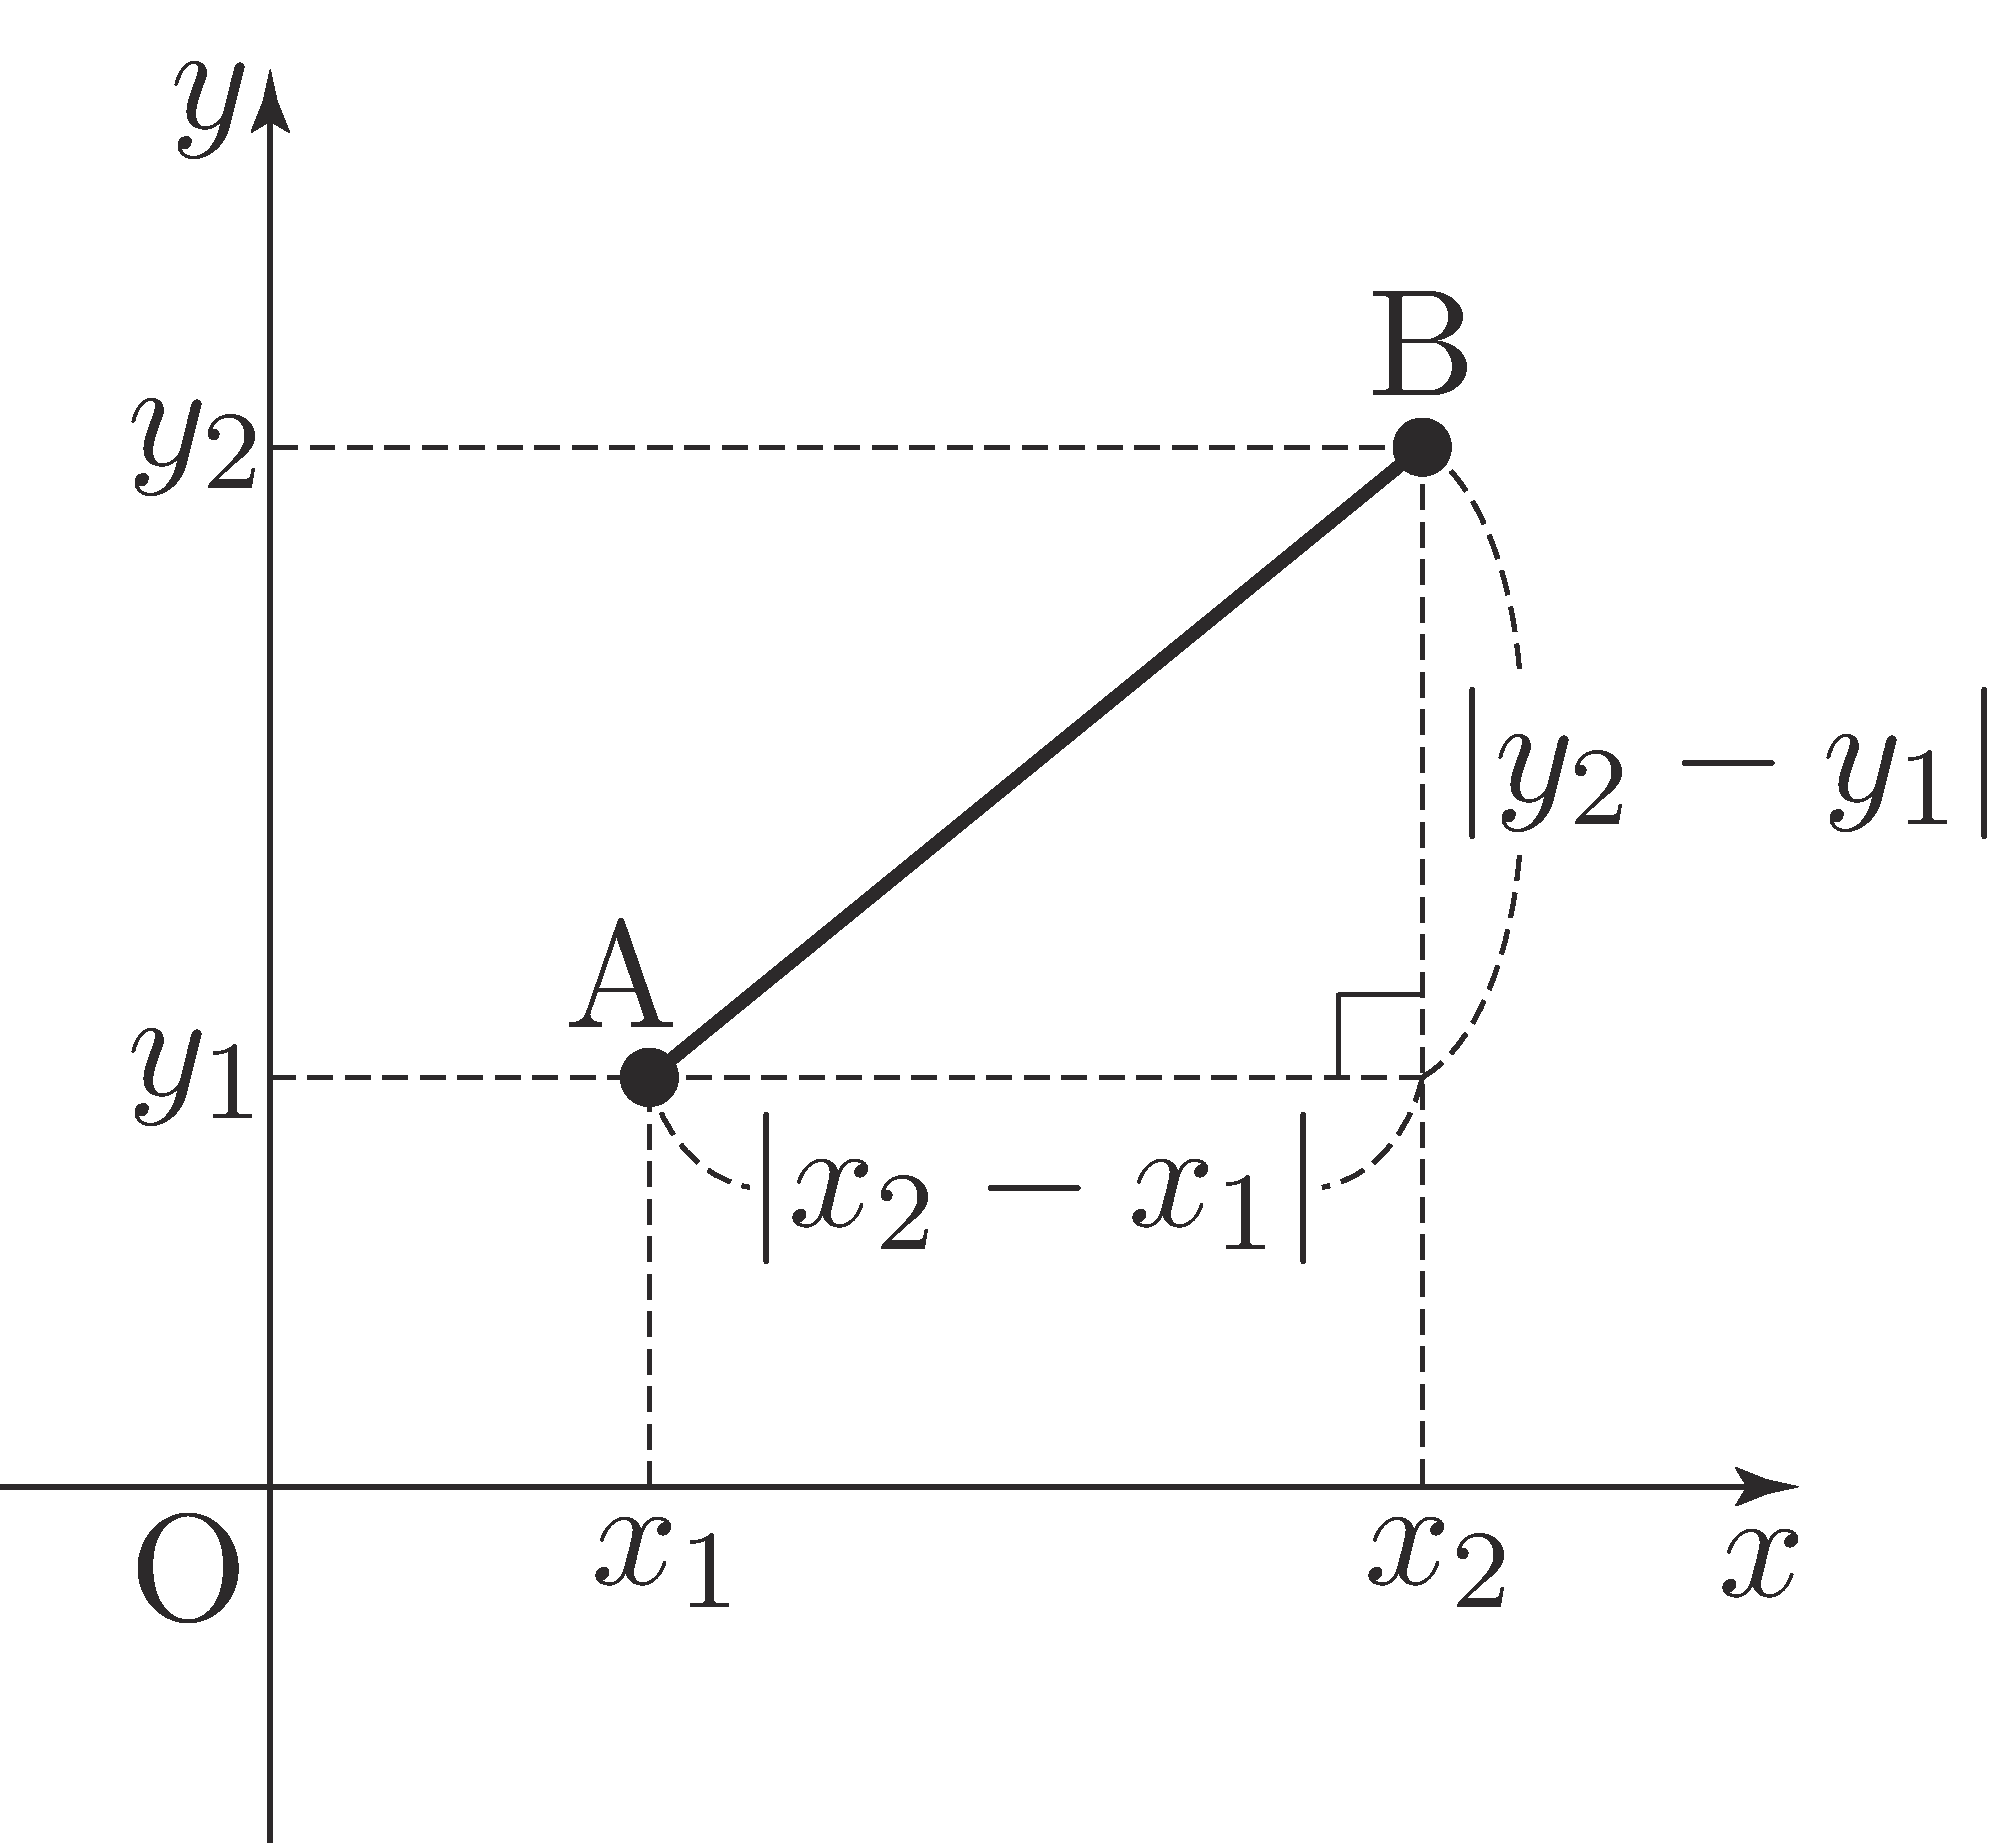
\includegraphics[scale=0.125]{pic0/pic144.pdf}\
\end{center}좌표평면에서 두 점 $\xy[A]{x_1}{y_1}$, $\xy[B]{x_2}{y_2}$ 사이의 거리 $\ovr{AB}$는 다음과 같습니다. \begin{align*}\ovr{AB} = \sqrt{(x_2 - x_1)^2 + (y_2 - y_1)^2}\end{align*}\\[-4.5em]
\section{내분점과 외분점}\term[내분]{좌표평면에서의 내분}{0}\term[외분]{좌표평면에서의 내분}{0}
\begin{center}
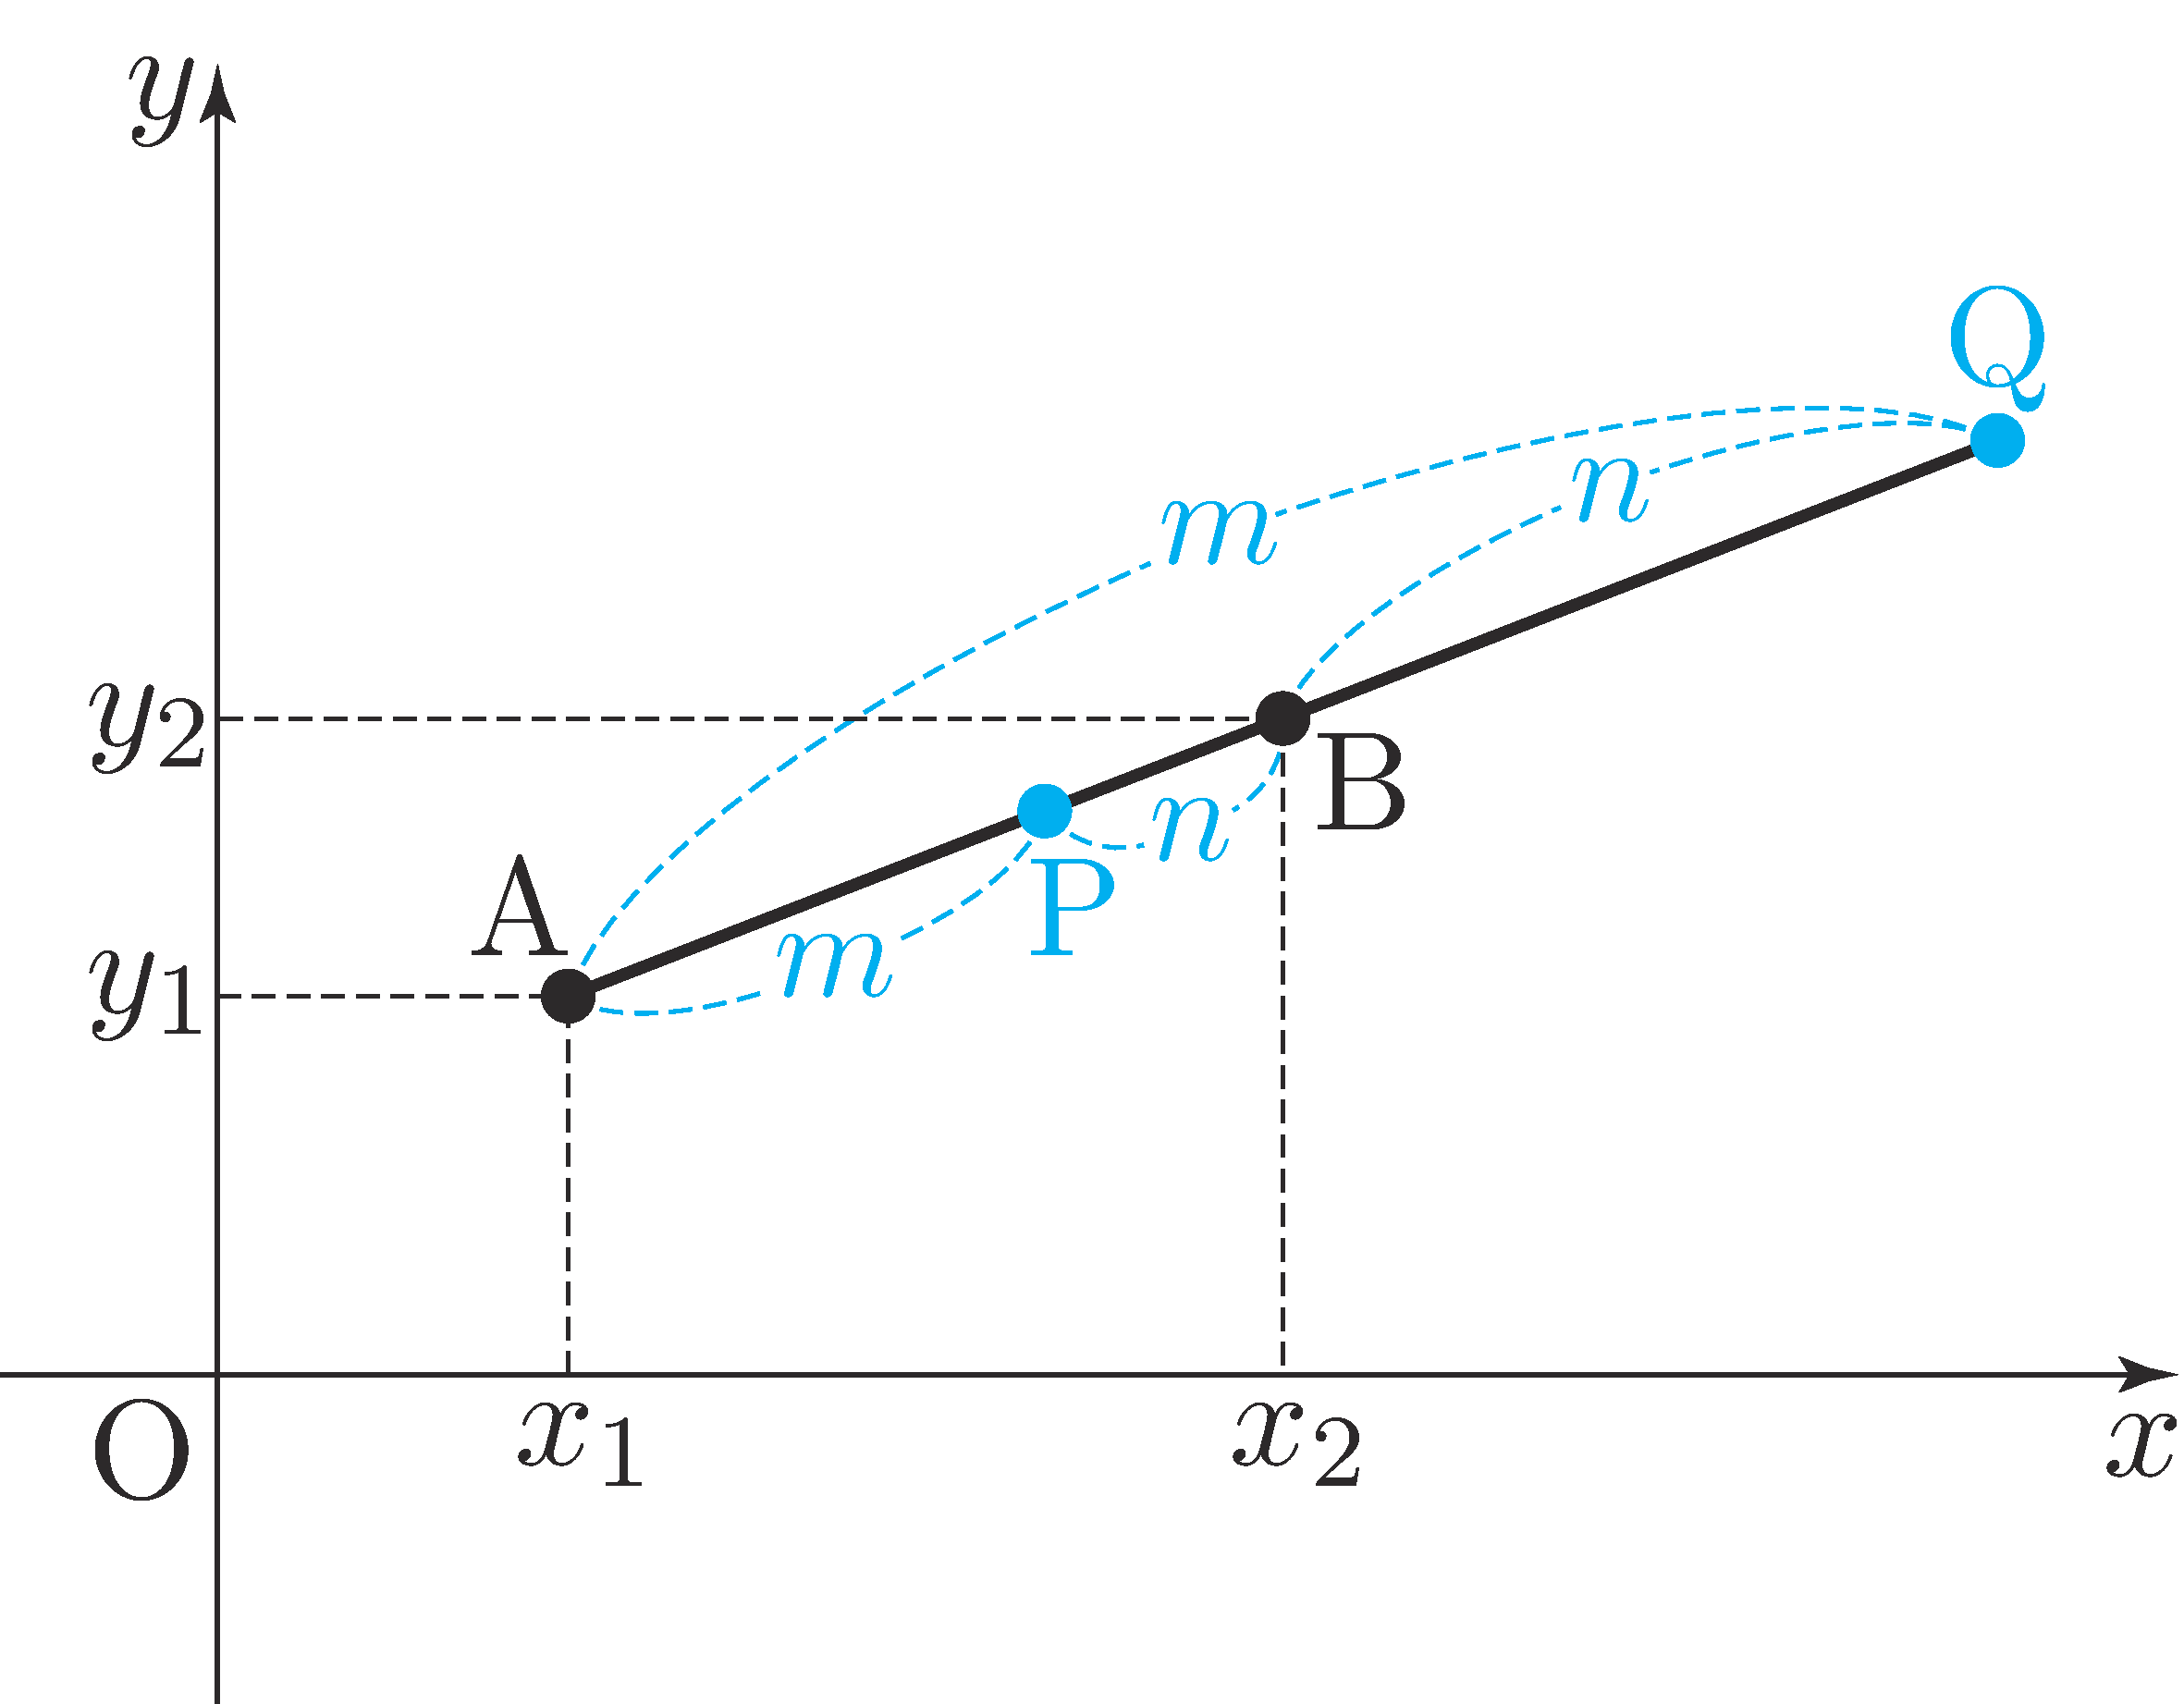
\includegraphics[scale=0.125]{pic0/pic145.pdf}\
\end{center}좌표평면에서 두 점 $\xy[A]{x_1}{y_1}$, $\xy[B]{x_2}{y_2}$에 대하여 선분 $\mrm{AB}$를 $m:n$으로 내분하는 점 $\mrm{P}$의 좌표와 $m:n$으로 외분하는 점 $\mrm{Q}$의 좌표는 각각 다음과 같습니다.\mn{외분할 때에는 $m\ne n$이어야 합니다.}{}\\[-1em]
\begin{align*}
  \xy[P]{\IDP{x_1}{x_2}{m}{n}}{\IDP{y_1}{y_2}{m}{n}},\quad
  \xy[Q]{\EDP{x_1}{x_2}{m}{n}}{\EDP{y_1}{y_2}{m}{n}}
\end{align*}\\[-4.5em]
\section{무게중심}\term[무게중심]{좌표평면}{0}
\begin{center}
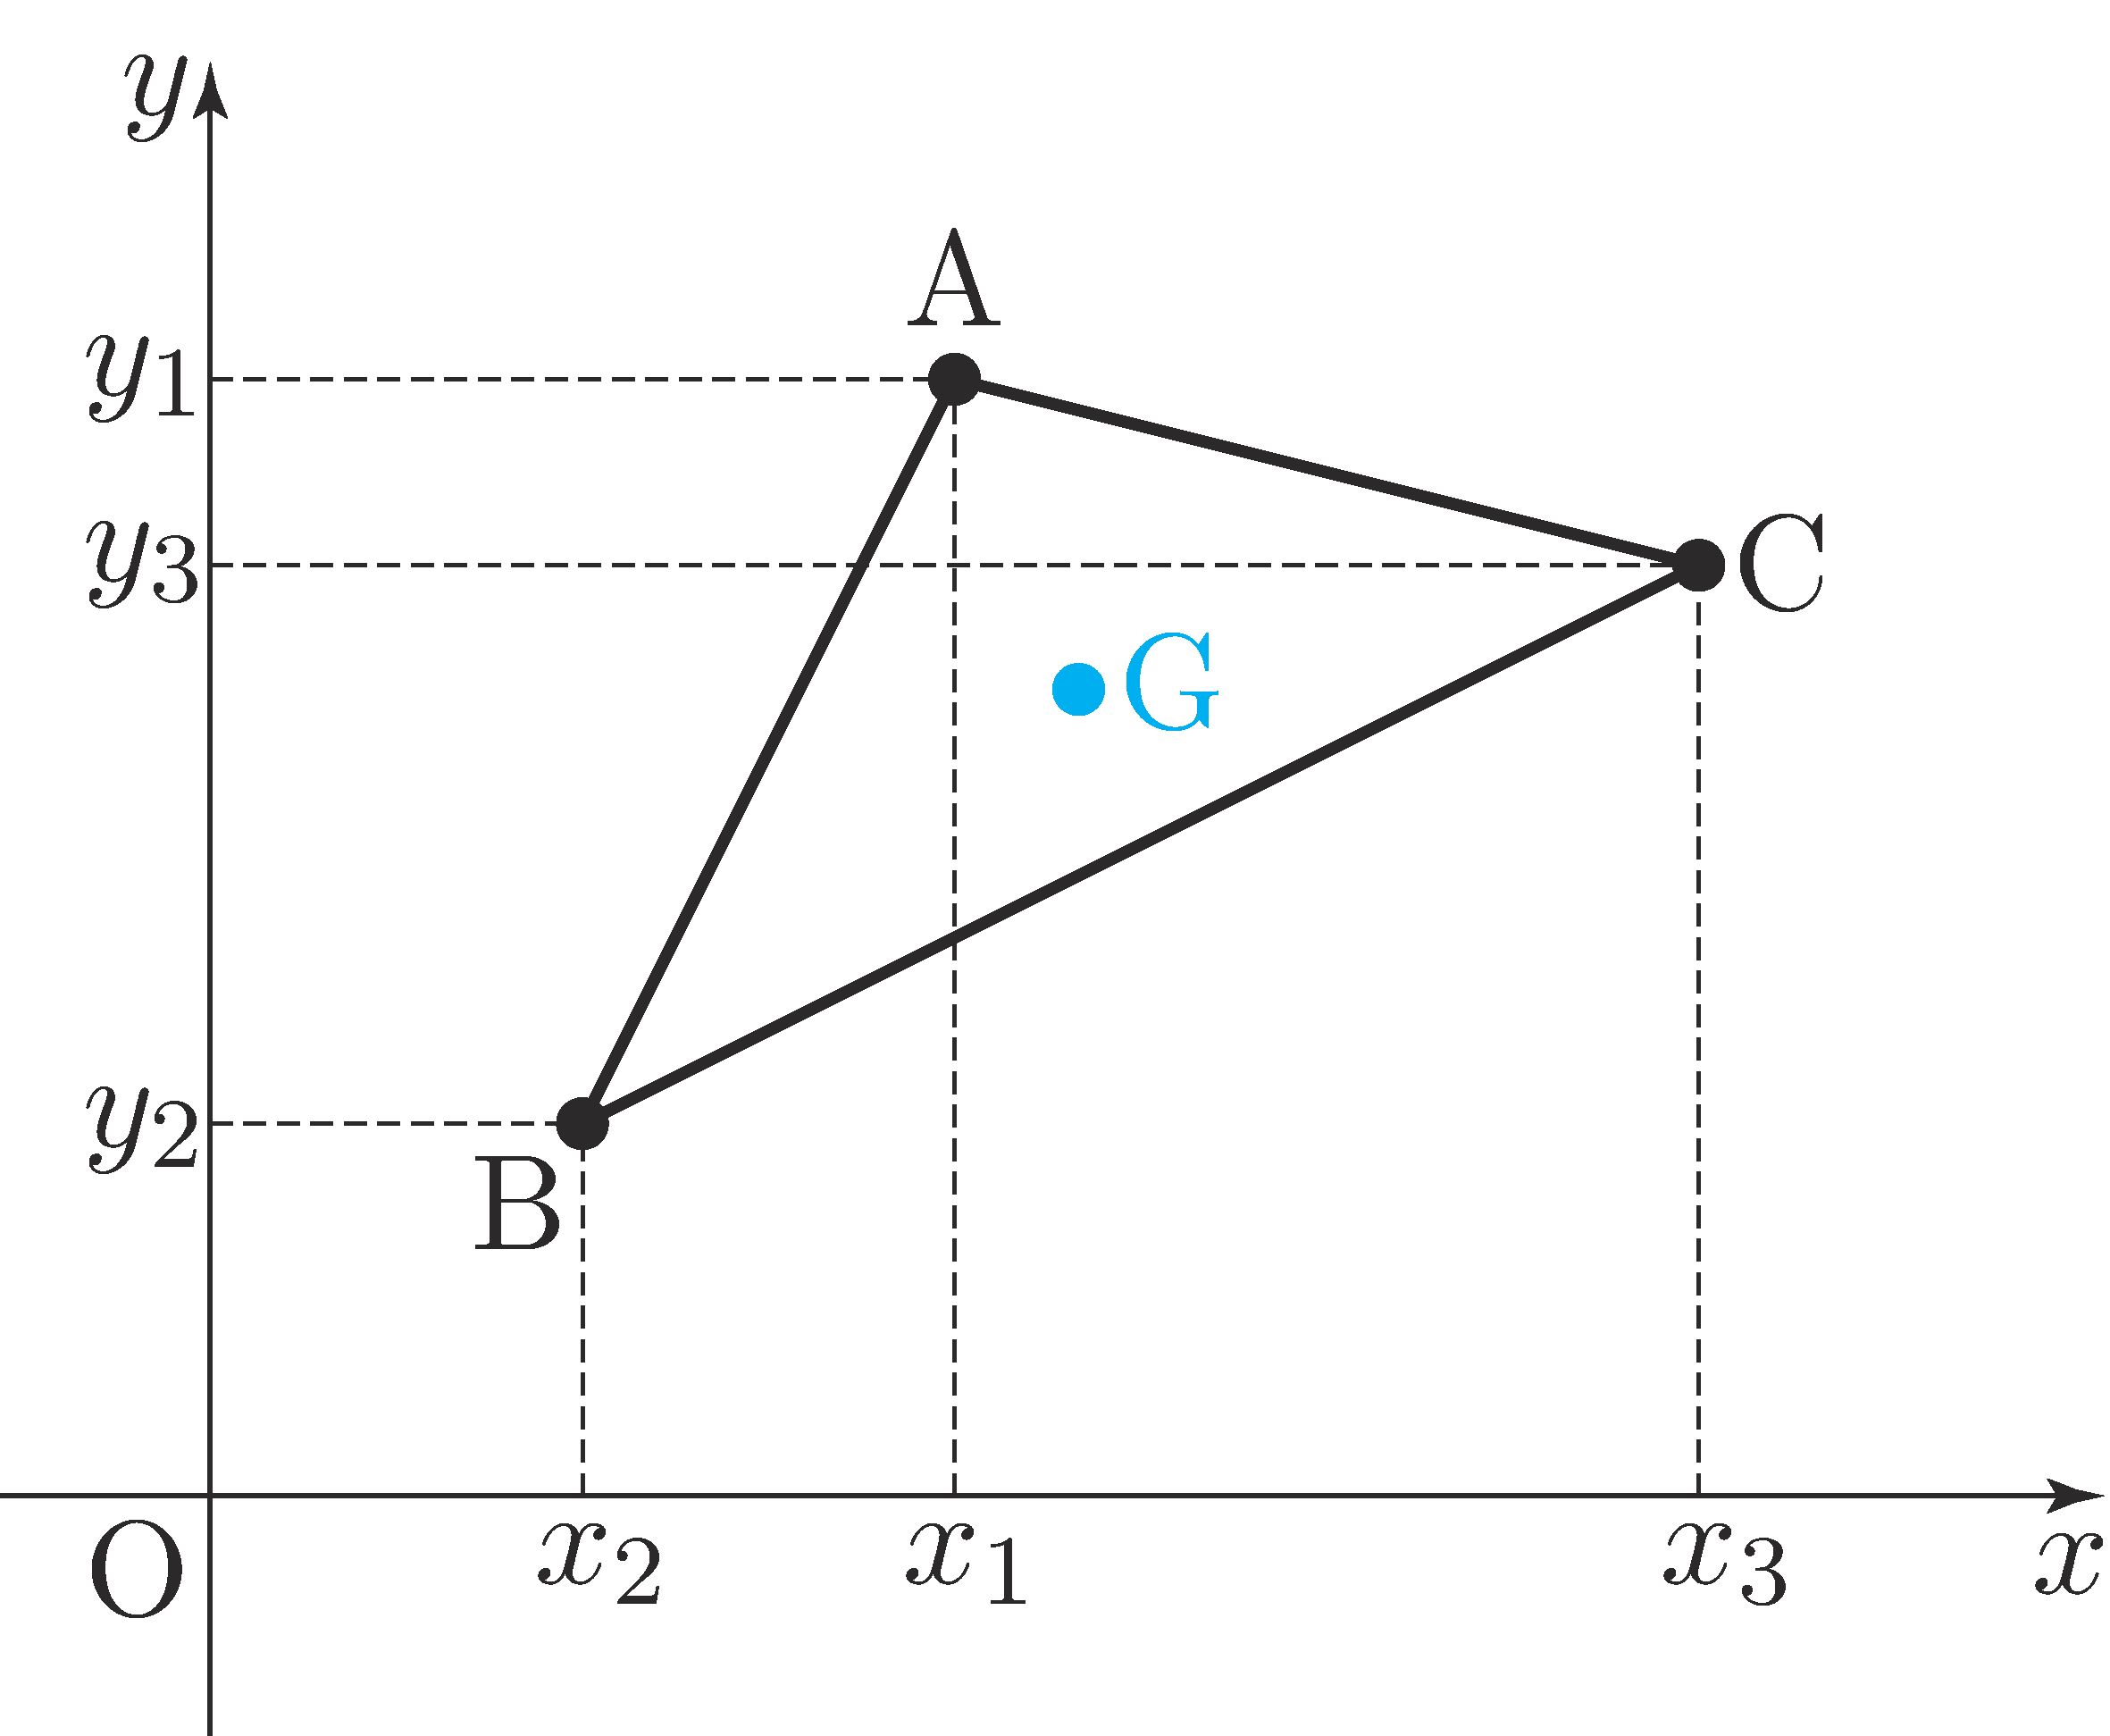
\includegraphics[scale=0.125]{pic0/pic146.pdf}\
\end{center}좌표평면에서 서로 다른 세 점 $\xy[A]{x_1}{y_1}$,  $\xy[B]{x_2}{y_2}$,  $\xy[C]{x_3}{y_3}$를 꼭짓점으로 하는 삼각형 $\mrm{ABC}$의 무게중심\mn[-5em]{삼각형의 무게중심은 각 꼭짓점과 마주보는 변의 중점을 이은 세 선분이 만나는 점입니다. 이때 각 선분이 무게중심에 의해 $1:2$로 내분된다는 특징이 있습니다.}{} $\mrm{G}$의 좌표는 다음과 같습니다. \begin{align*}\xy[G]{\dfrac{x_1 + x_2 + x_3}{3}}{\dfrac{y_1 + y_2 + y_3}{3}}\end{align*}
\clearpage
\section{도형의 방정식}
\subsection{직선의 방정식}\term[직선의 방정식]{좌표평면}{0}
\begin{center}
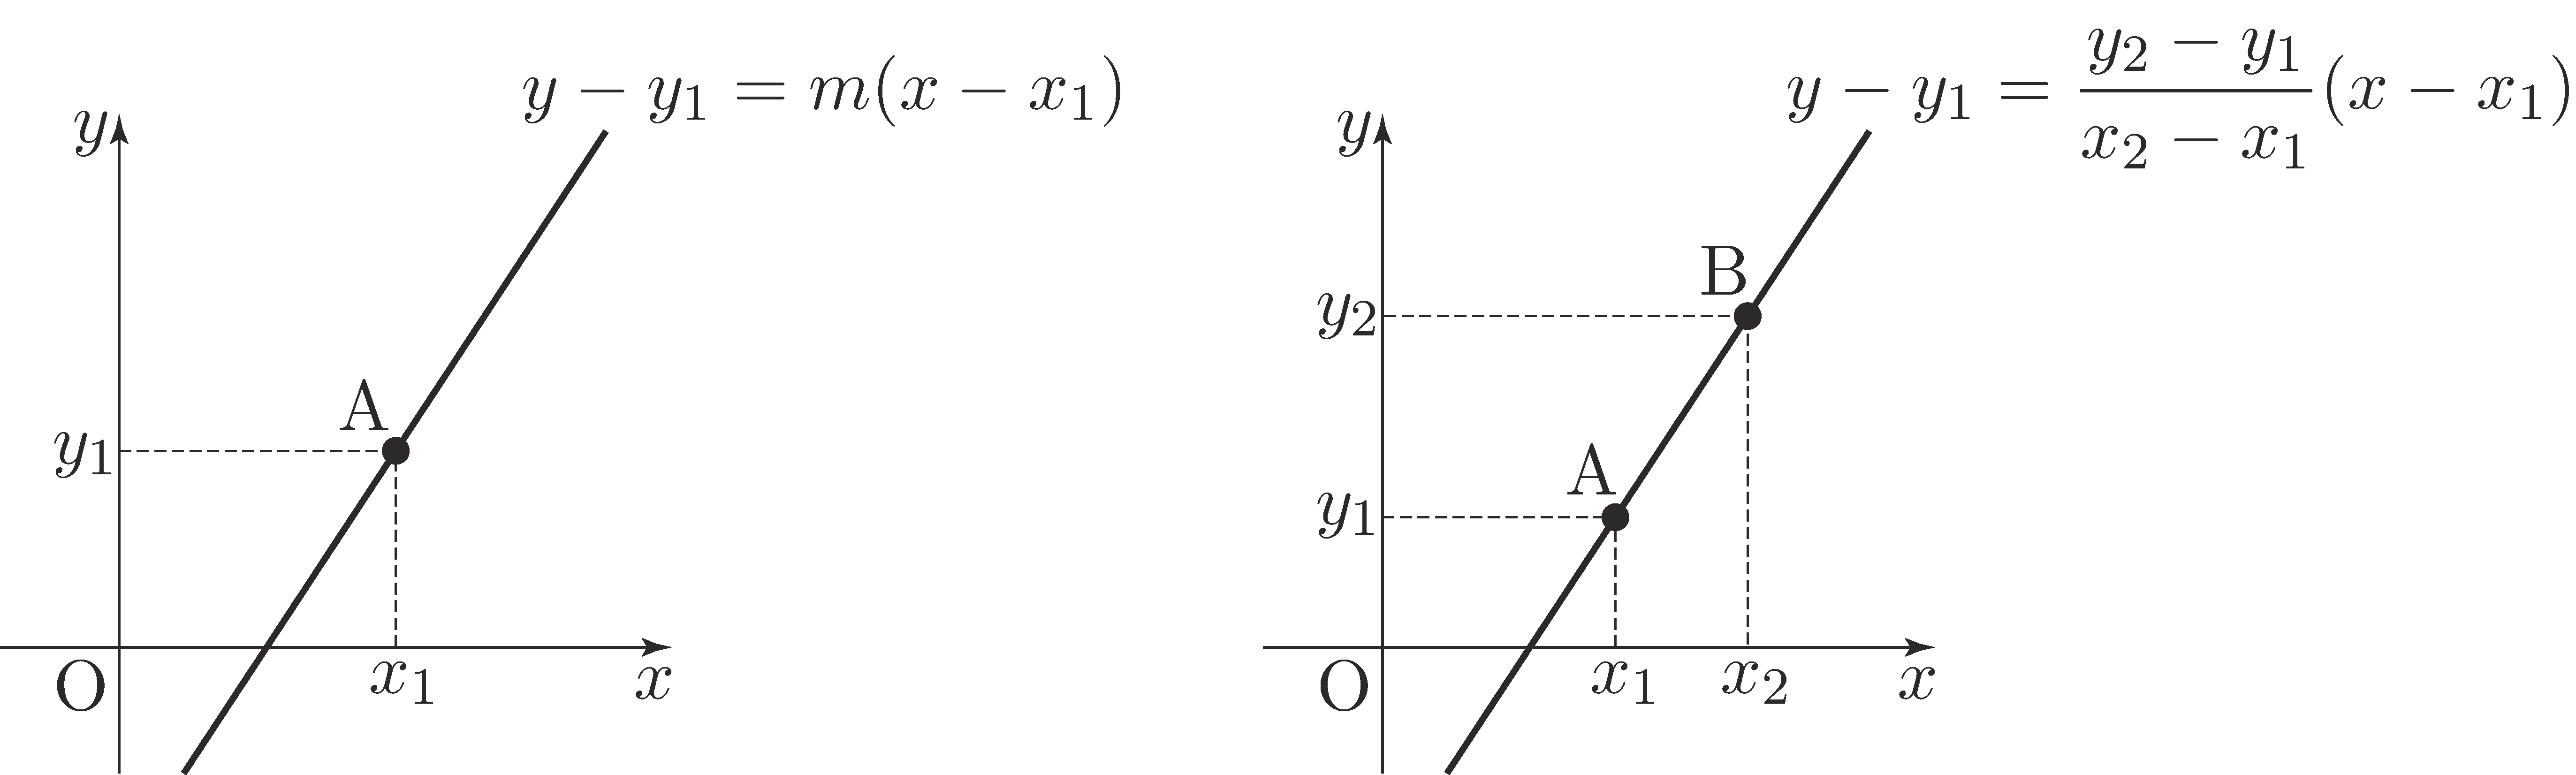
\includegraphics[scale=0.125]{pic0/pic147.pdf}
\end{center}좌표평면에서 한 점 $\xy[A]{x_1}{y_1}$을 지나고 기울기가 $m$인 직선의 방정식은 다음과 같습니다. \begin{align*}y-y_1 = m (x-x_1)\end{align*}
좌표평면에서 두 점 $\xy[A]{x_1}{y_1}$, $\xy[B]{x_2}{y_2}$를 지나는 직선의 방정식은 다음과 같습니다.
\begin{alignat*}{2}
  y-y_1 &= \dfrac{y_2-y_1}{x_2-x_1}(x-x_1) \quad &&(x_1 \ne x_2)\\
  x&=x_1 \quad &&(x_1 = x_2)
\end{alignat*}

한편 직선의 방정식의 일반적인 식은 일차방정식 $ax+by+c=0$의 꼴이며 이때 $a\ne0$ 또는 $b\ne0$입니다.
\subsubsection{두 직선의 평행과 수직}\term[평행!좌표평면에서]{두 직선의 평행조건}{0}\term[수직!좌표평면에서]{두 직선의 수직조건}{0}

\begin{figure}[h]
  \centering
  \subfloat[][]{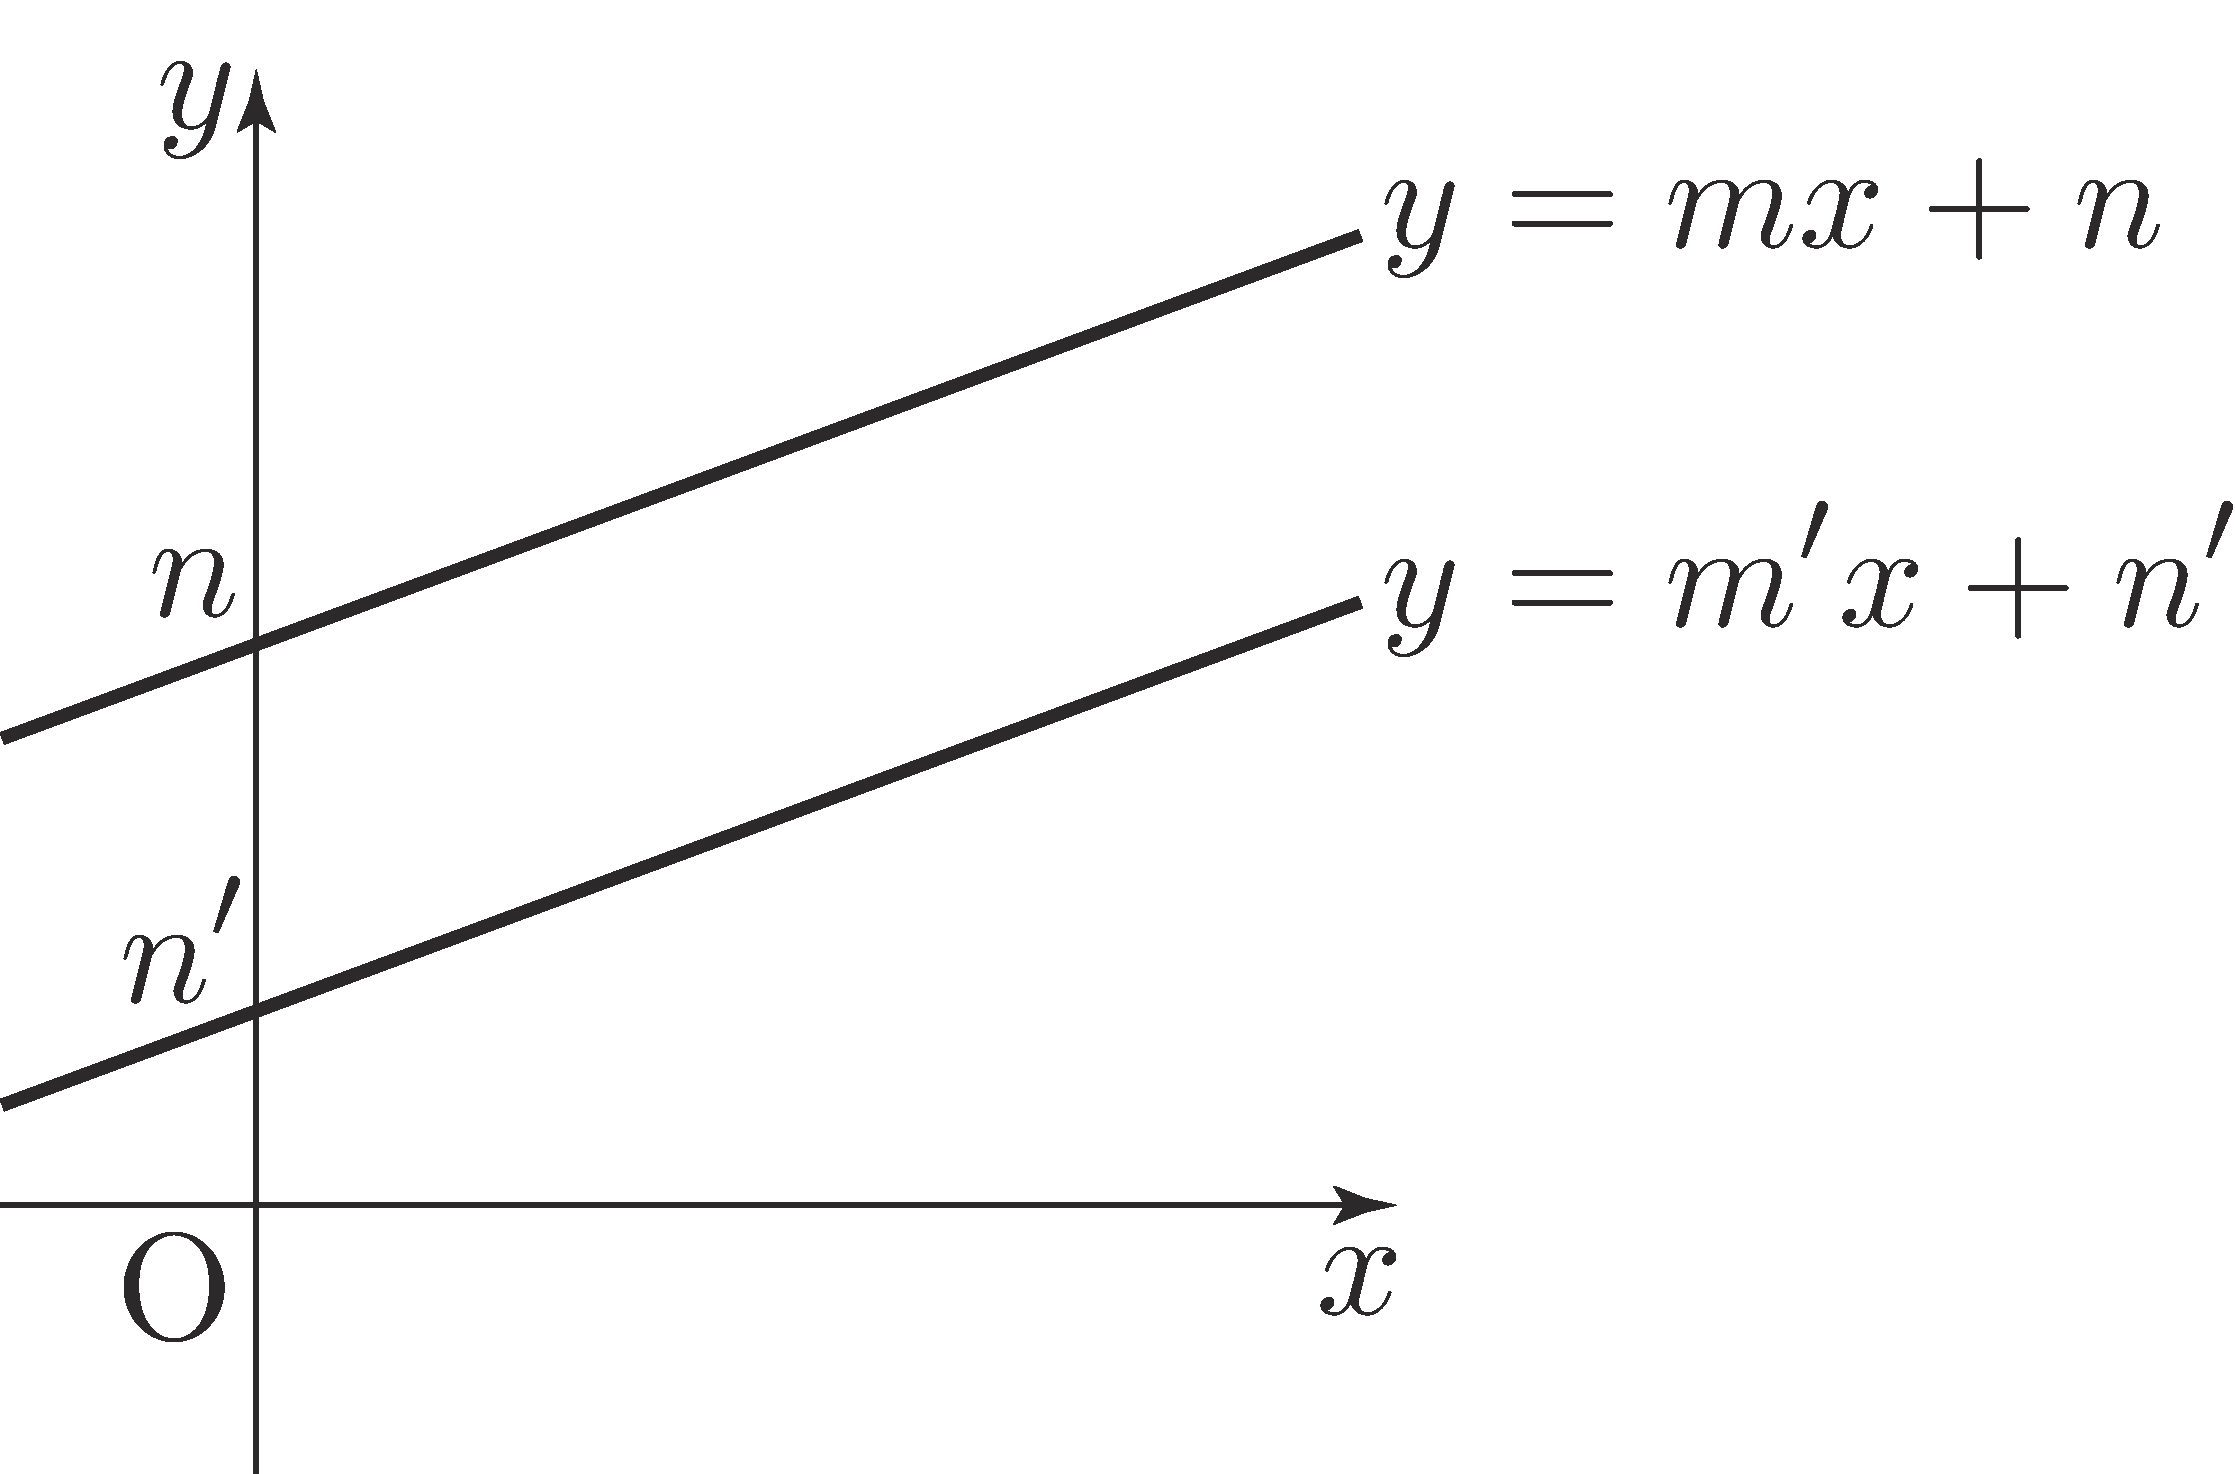
\includegraphics[scale=.125]{pic0/pic148_1.pdf}}
  \qquad
  \subfloat[][]{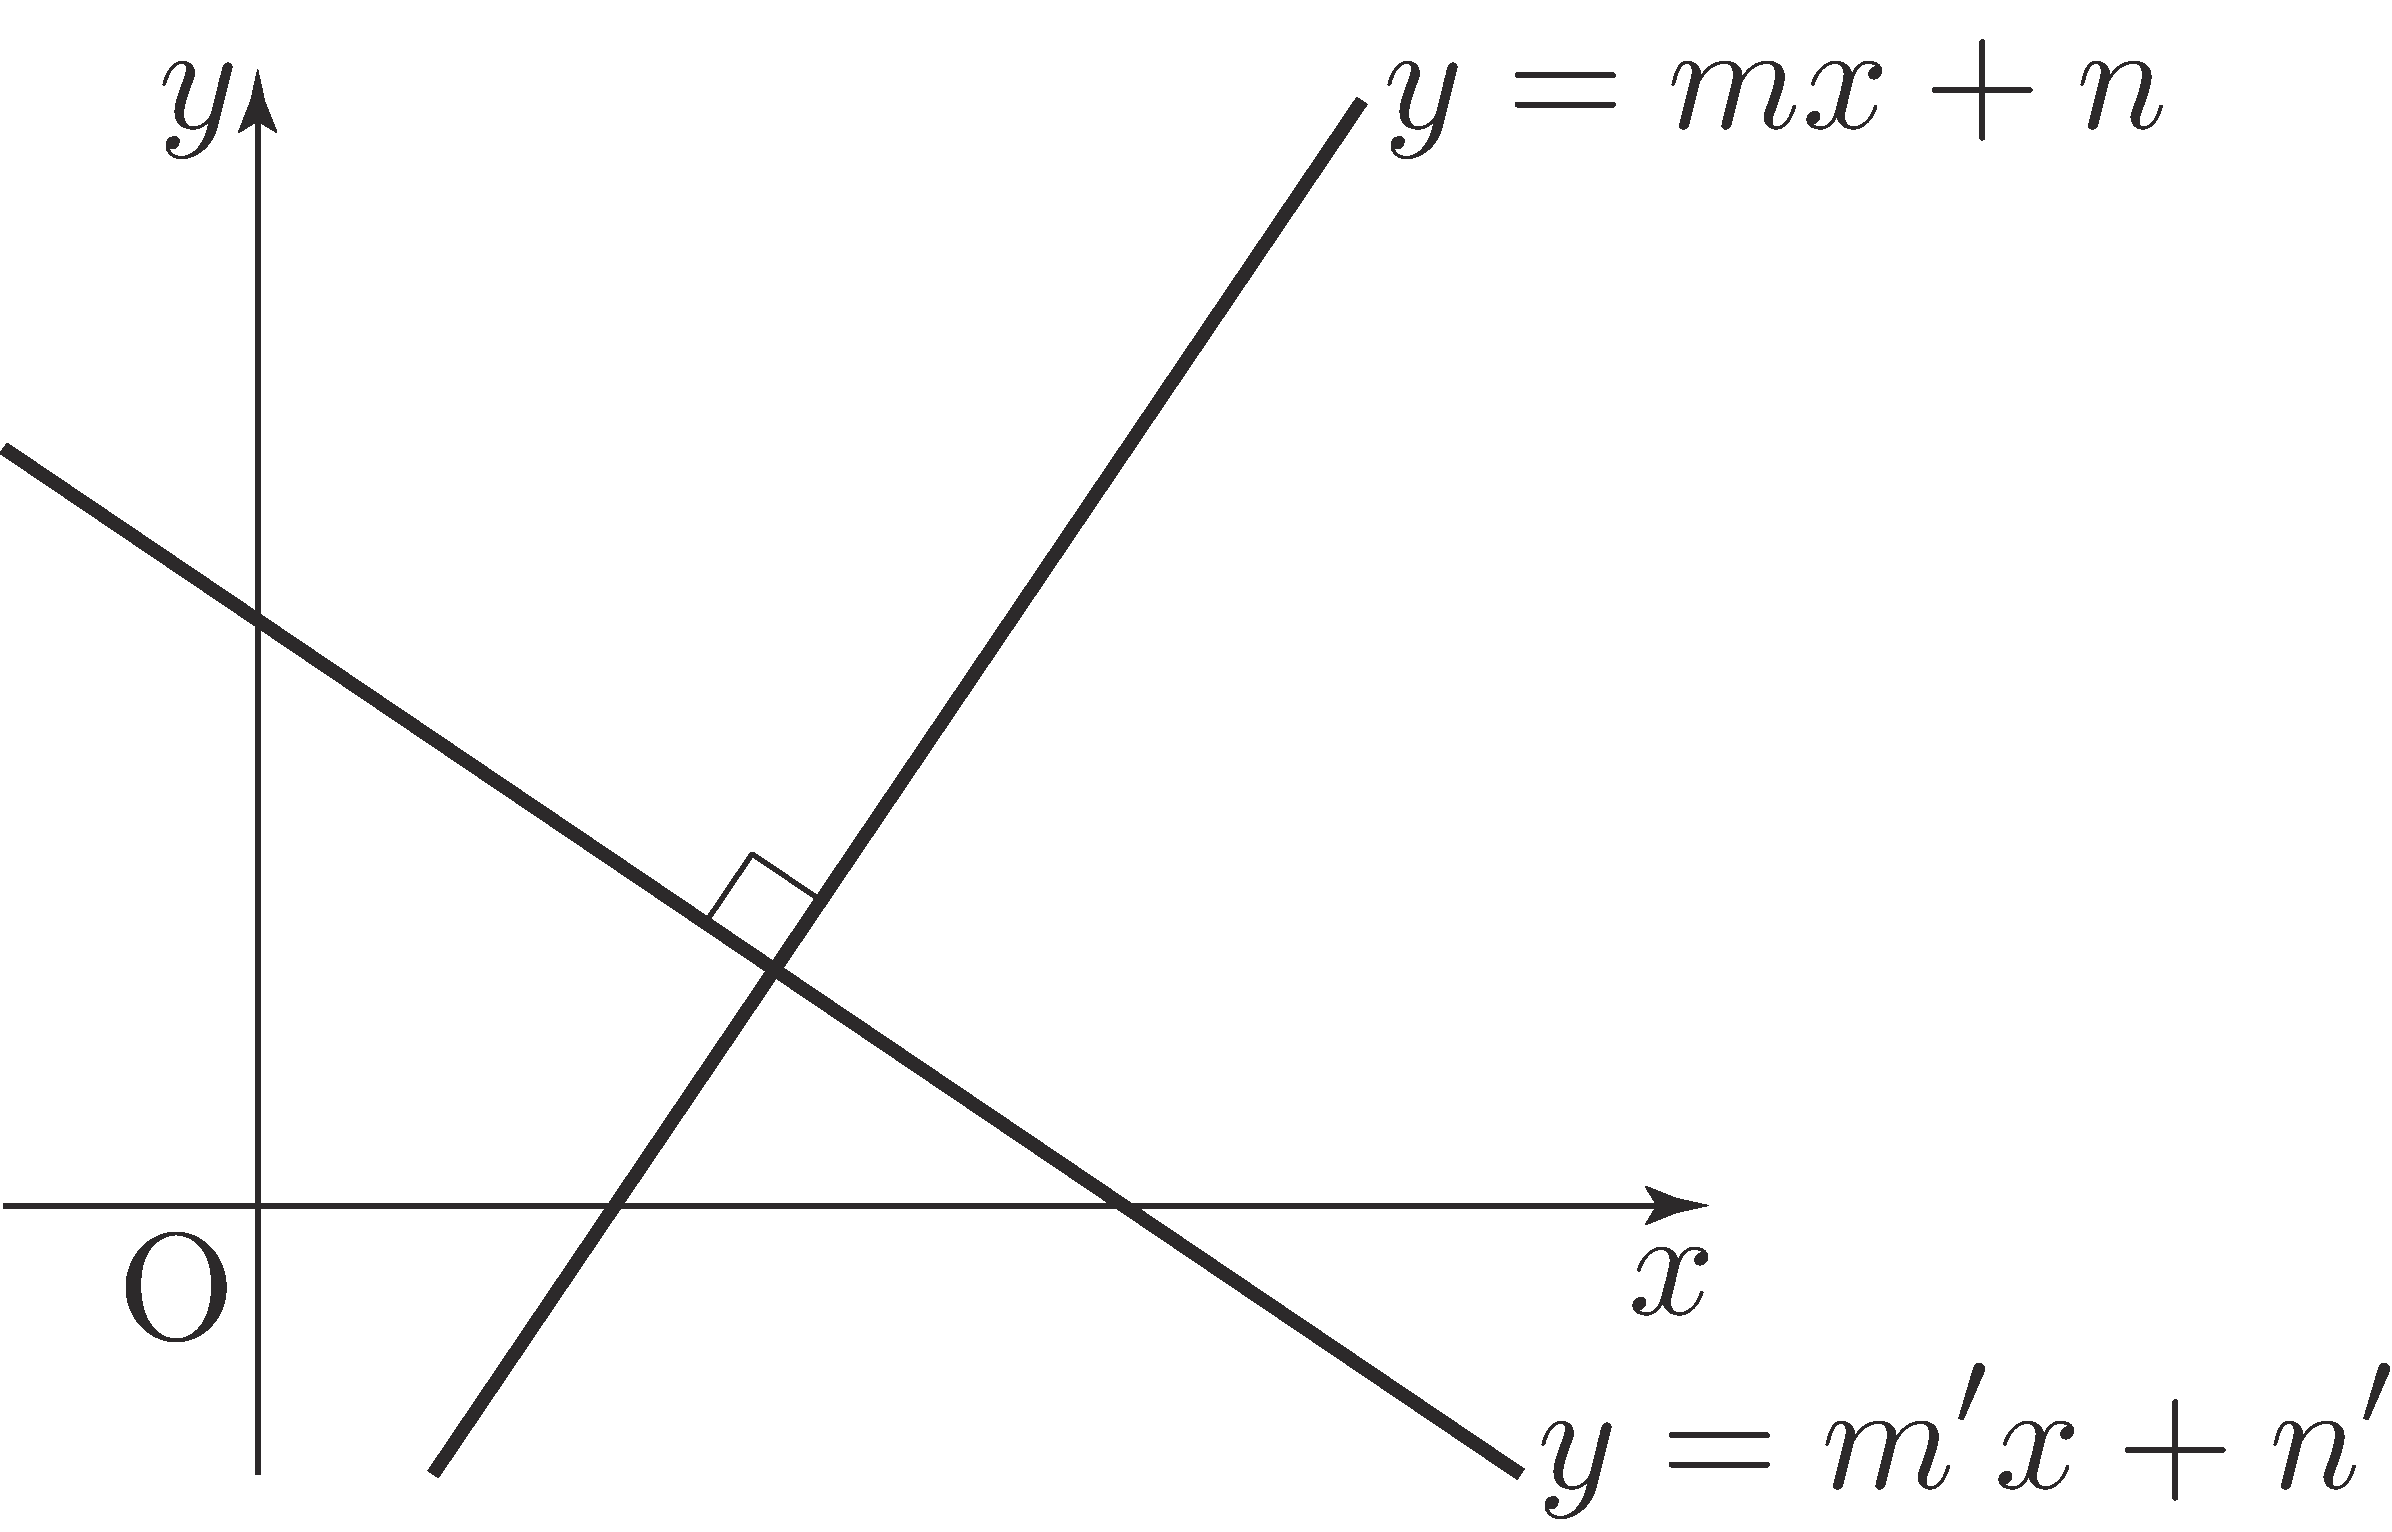
\includegraphics[scale=.125]{pic0/pic148_2.pdf}}
\end{figure}

(a)와 같이 두 직선 $y=mx+n$, $y=m'x+n'$이 서로 평행하면 $m=m'$, $n \ne n'$입니다. 반대로 $m=m'$, $n \ne n'$이면 두 직선이 평행합니다. (b)와 같이 $m \ne 0$, $m' \ne 0$이고 두 직선이 서로 수직이면 $mm' = -1$입니다. 반대로 $mm'=-1$이면 두 직선이 서로 수직입니다.

\subsubsection{점과 직선 사이의 거리}\term[거리!좌표평면]{점과 직선 사이의 거리}{0}
점 $\xy[P]{x_1}{y_1}$과 직선 $ax+by+c=0$ 사이의 거리 $d$는 다음과 같습니다.
\begin{align*} d = \dfrac{\abs{ax_1+by_1+c}}{\sqrt{a^2+b^2}} \end{align*}
\clearpage
\subsection{원의 방정식}\term[원!좌표평면]{원의 방정식}{0}
\begin{figure}[h]\centering \subfloat[][]{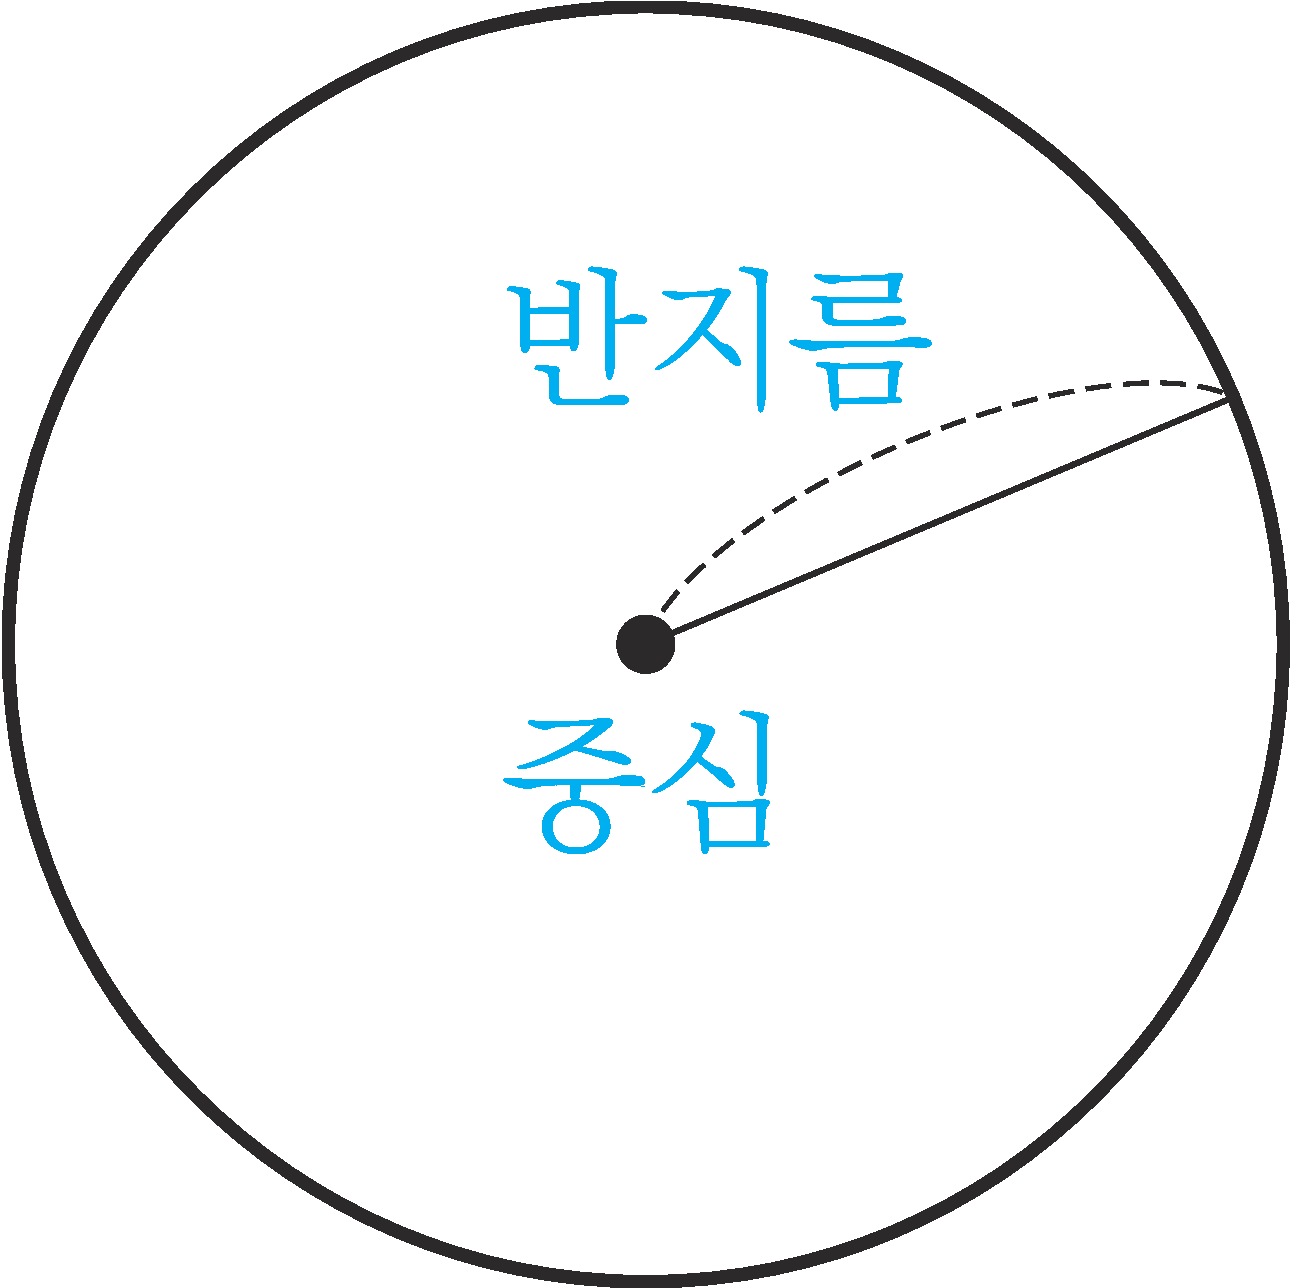
\includegraphics[scale=0.125]{pic0/pic162_1.pdf}}\
\qquad
\centering \subfloat[][]{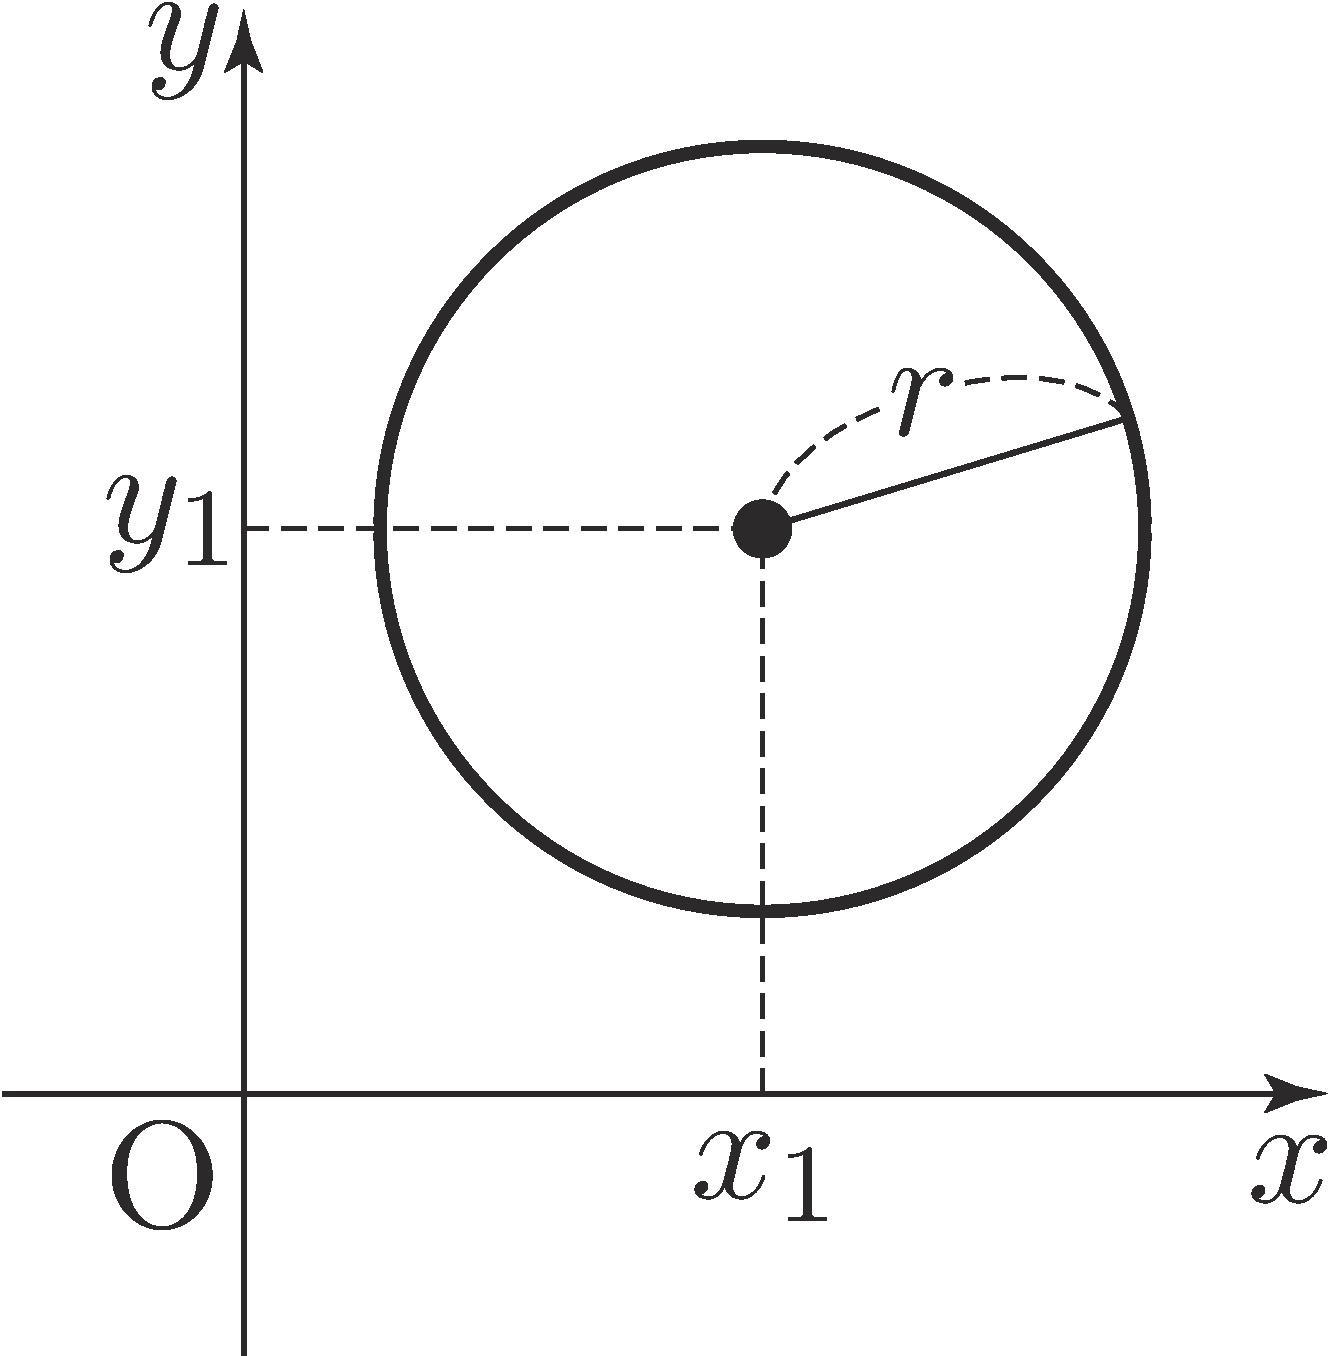
\includegraphics[scale=0.125]{pic0/pic162_2.pdf}}\
\end{figure}

(a)와 같이 평면에서 한 정점으로부터 일정한 거리에 있는 점 전체의 집합을 \term{원}{}이라고 합니다. 이때 정점을 원의 \term[원]{중심}{2}, 원의 중심과 원 위의 한 점을 이은 선분을 원의 \term[원]{반지름}{2}이라고 합니다. (b)와 같이 좌표평면에서 중심의 좌표가 $\xy[C]{x_1}{y_1}$이고 반지름의 길이가 $r$인 원의 방정식은 다음과 같습니다.
\begin{align*} (x-x_1)^2 + (y-y_1)^2 = r^2 \end{align*}

한편 원의 방정식의 일반적인 식은 이차방정식 $x^2 + y^2 + Ax + By + C = 0$의 꼴이며 이때 $A^2 + B^2 - 4C > 0$입니다.

\subsubsection{원과 직선의 위치관계}\term[원!좌표평면]{원과 직선의 위치관계}{0}
\begin{center}
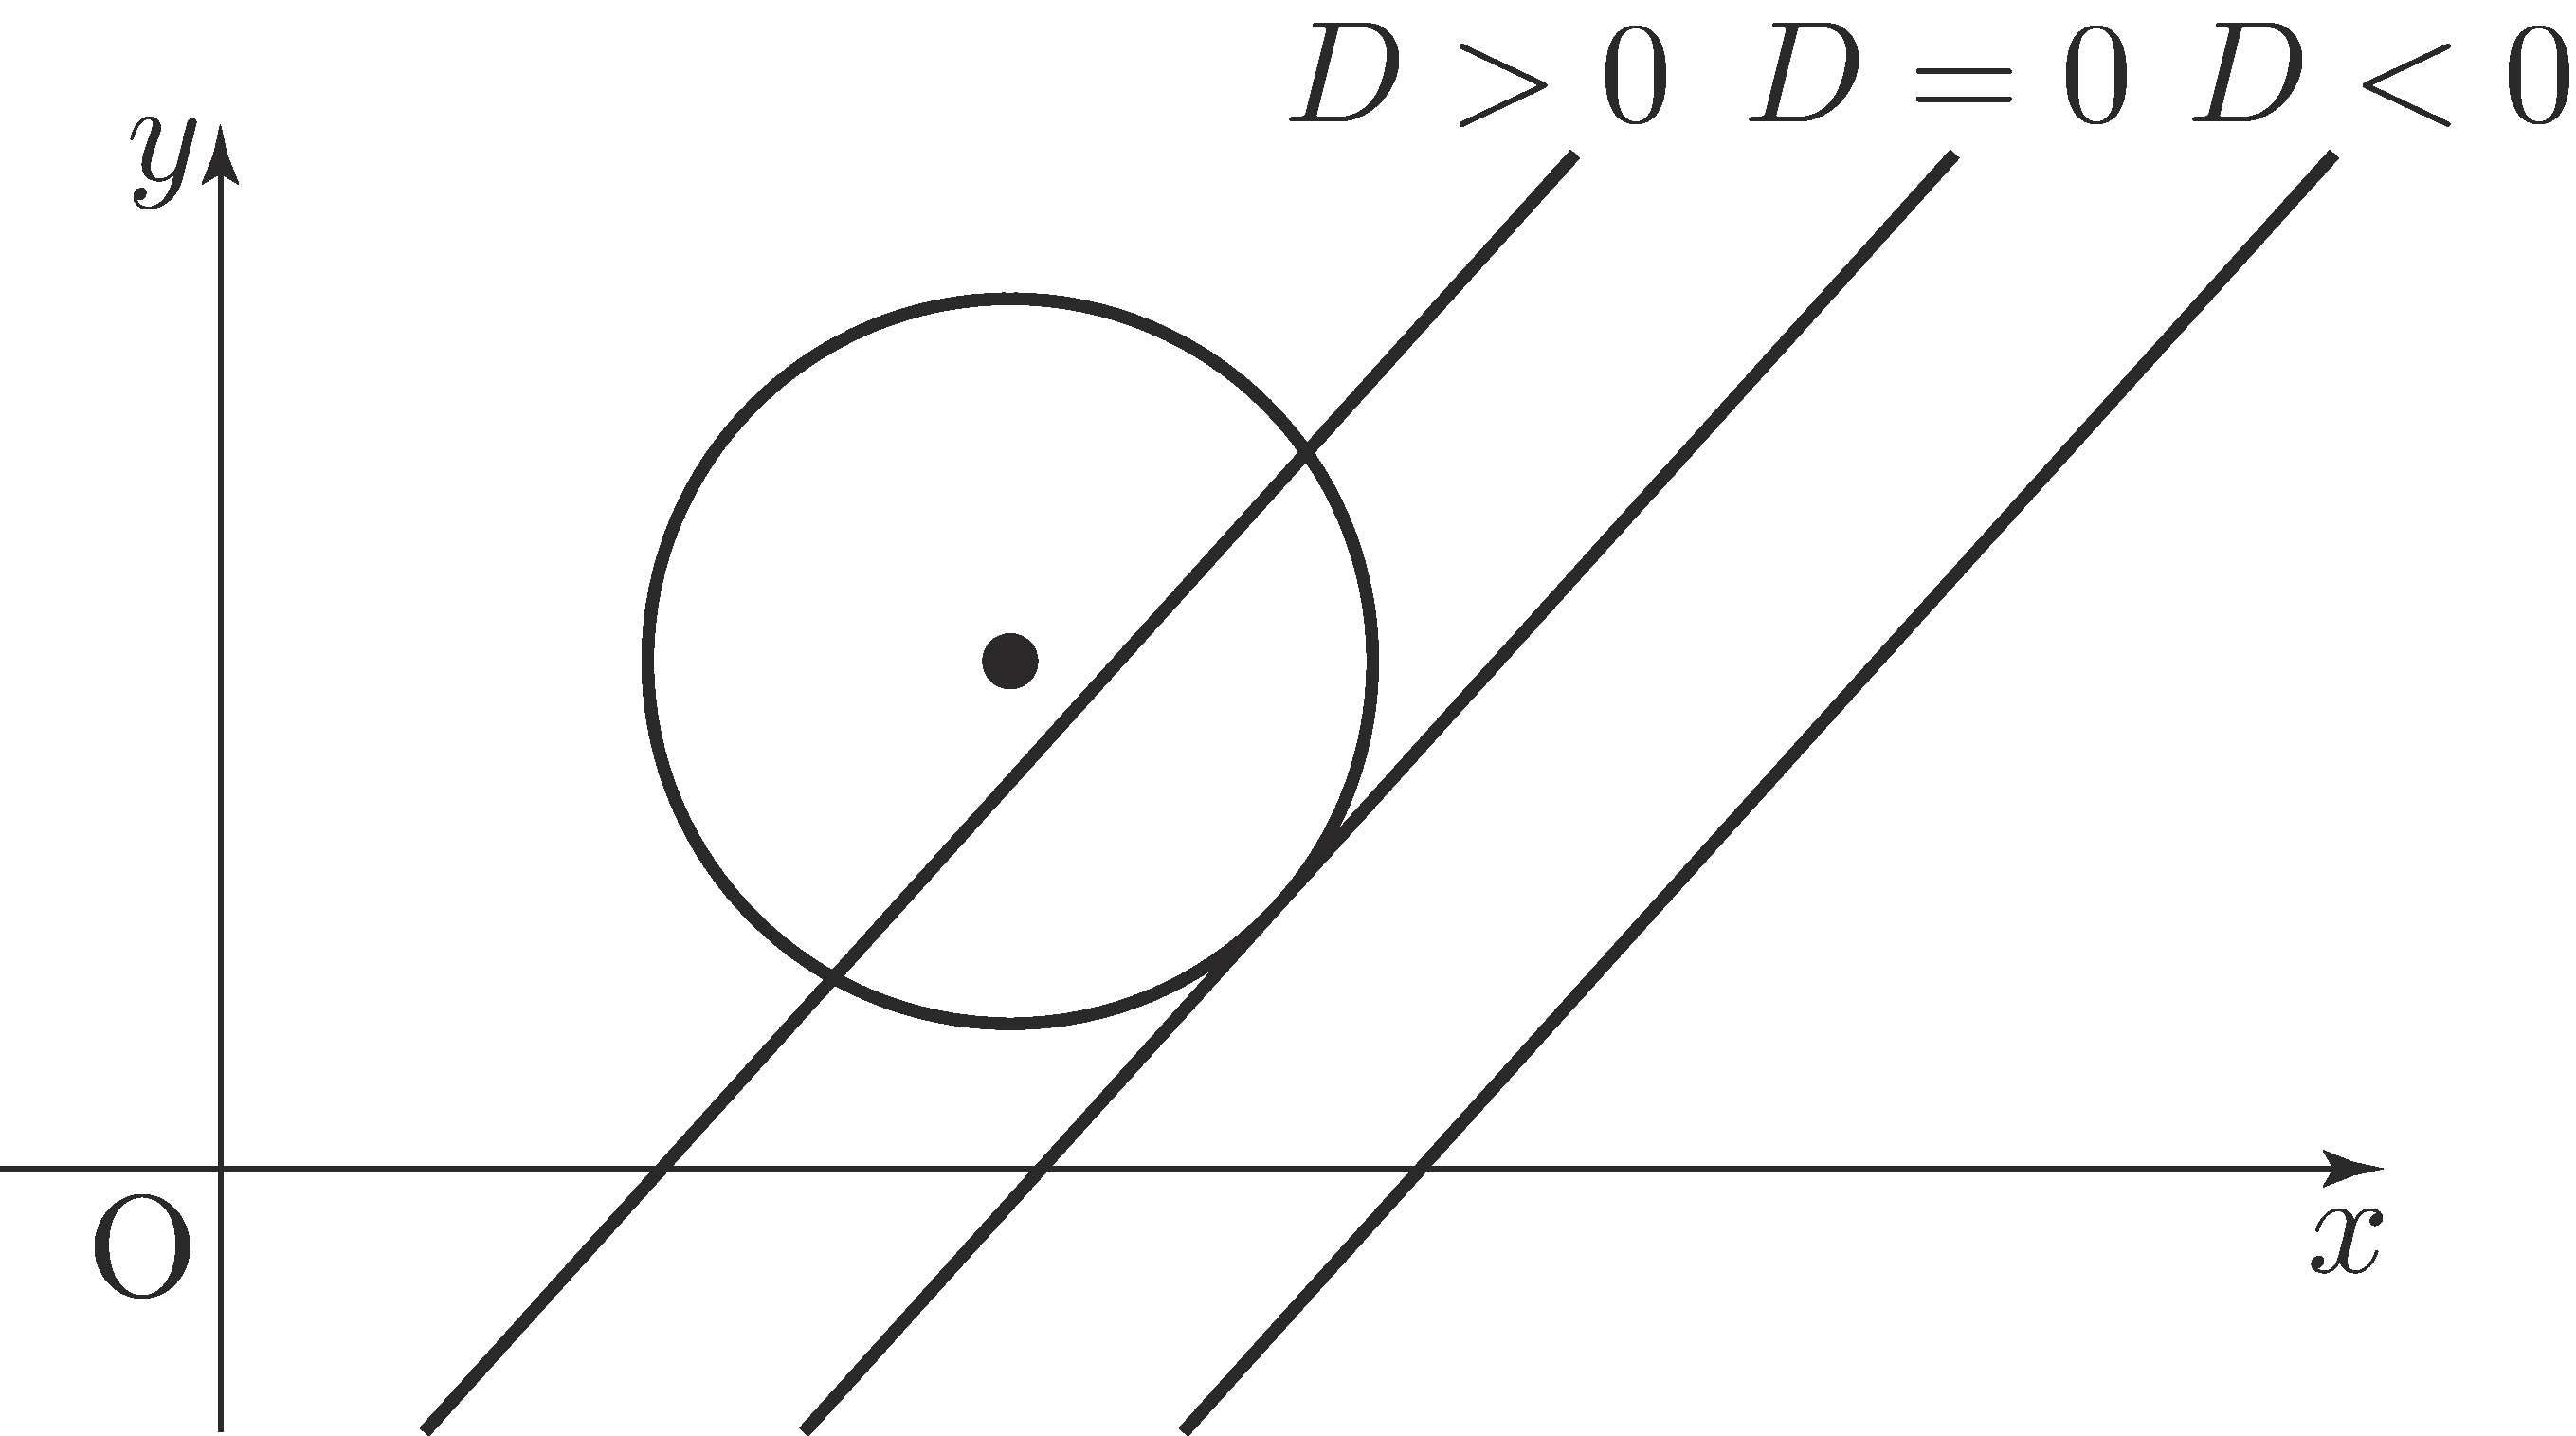
\includegraphics[scale=0.125]{pic0/pic163.pdf}\
\end{center}원 $x^2 + y^2 = r^2$과 직선 $y=mx+n$의 교점의 개수는 두 식을 연립한 이차방정식의 판별식 $D$의 부호에 따라 달라집니다. 반대로, 교점의 개수에 따라 $D$의 부호가 달라집니다.
\begin{justbox}
  \begin{enumerate}[label=\onum*]
    \item $D>0$ : 서로 다른 두 점에서 만난다.
    \item $D=0$ : 한 점에서 만난다. (접한다)
    \item $D<0$ : 만나지 않는다.
  \end{enumerate}
\end{justbox}
\clearpage
\section{평행이동과 대칭이동}

\subsection{평행이동}\term{평행이동}{0}
\begin{center}
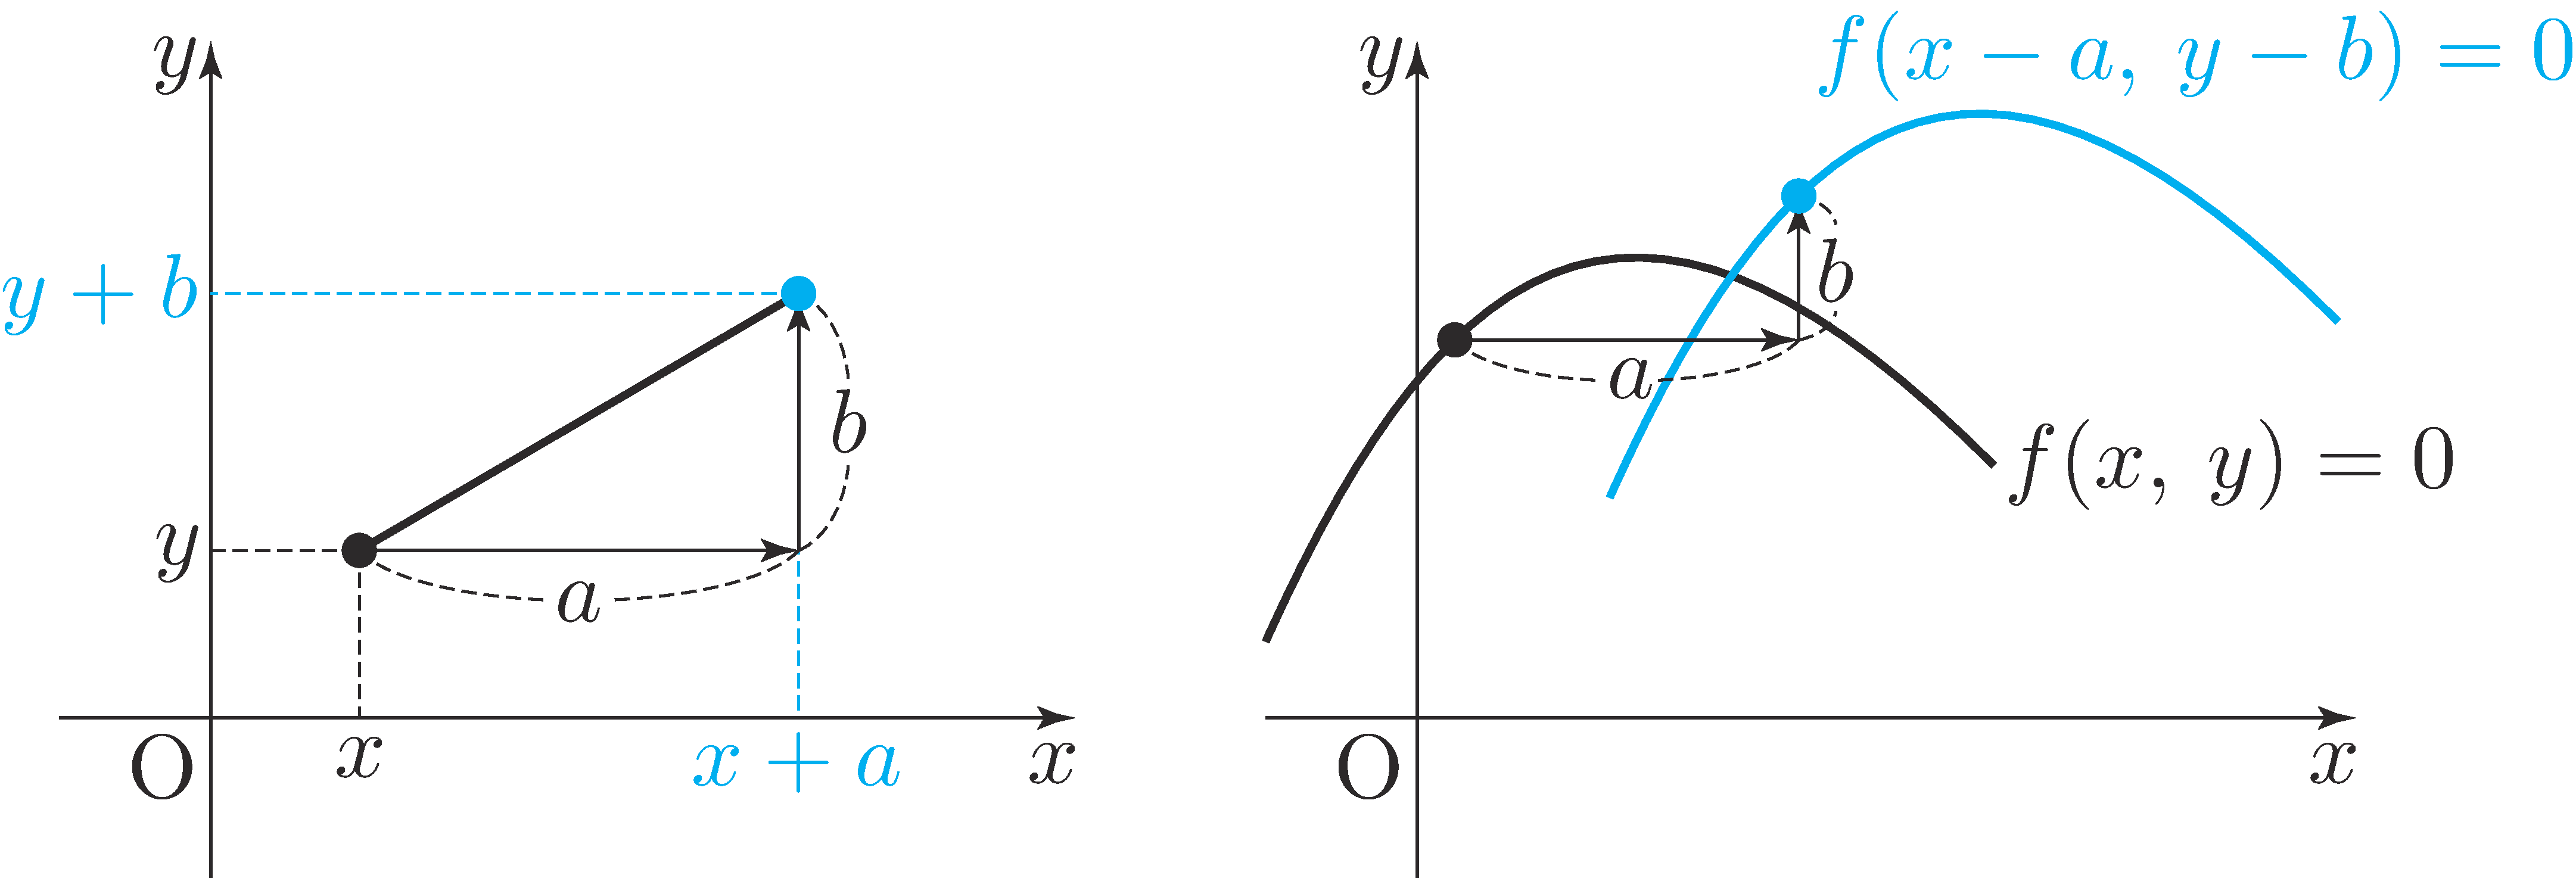
\includegraphics[scale=0.125]{pic0/pic149.pdf}
\end{center} 좌표가 $\xy{x}{y}$인 점을 $x$축 방향으로 $a$만큼, $y$축 방향으로 $b$만큼 평행이동한 점의 좌표는 $\xy{x+a}{y+b}$입니다. 도형 $f(x,\:y)=0$를 $x$축 방향으로 $a$만큼, $y$축 방향으로 $b$만큼 평행이동한 도형의 방정식은 $f(x-a,\:y-b)=0$입니다.

\subsection{대칭이동}\term{대칭이동}{0}
\begin{center}
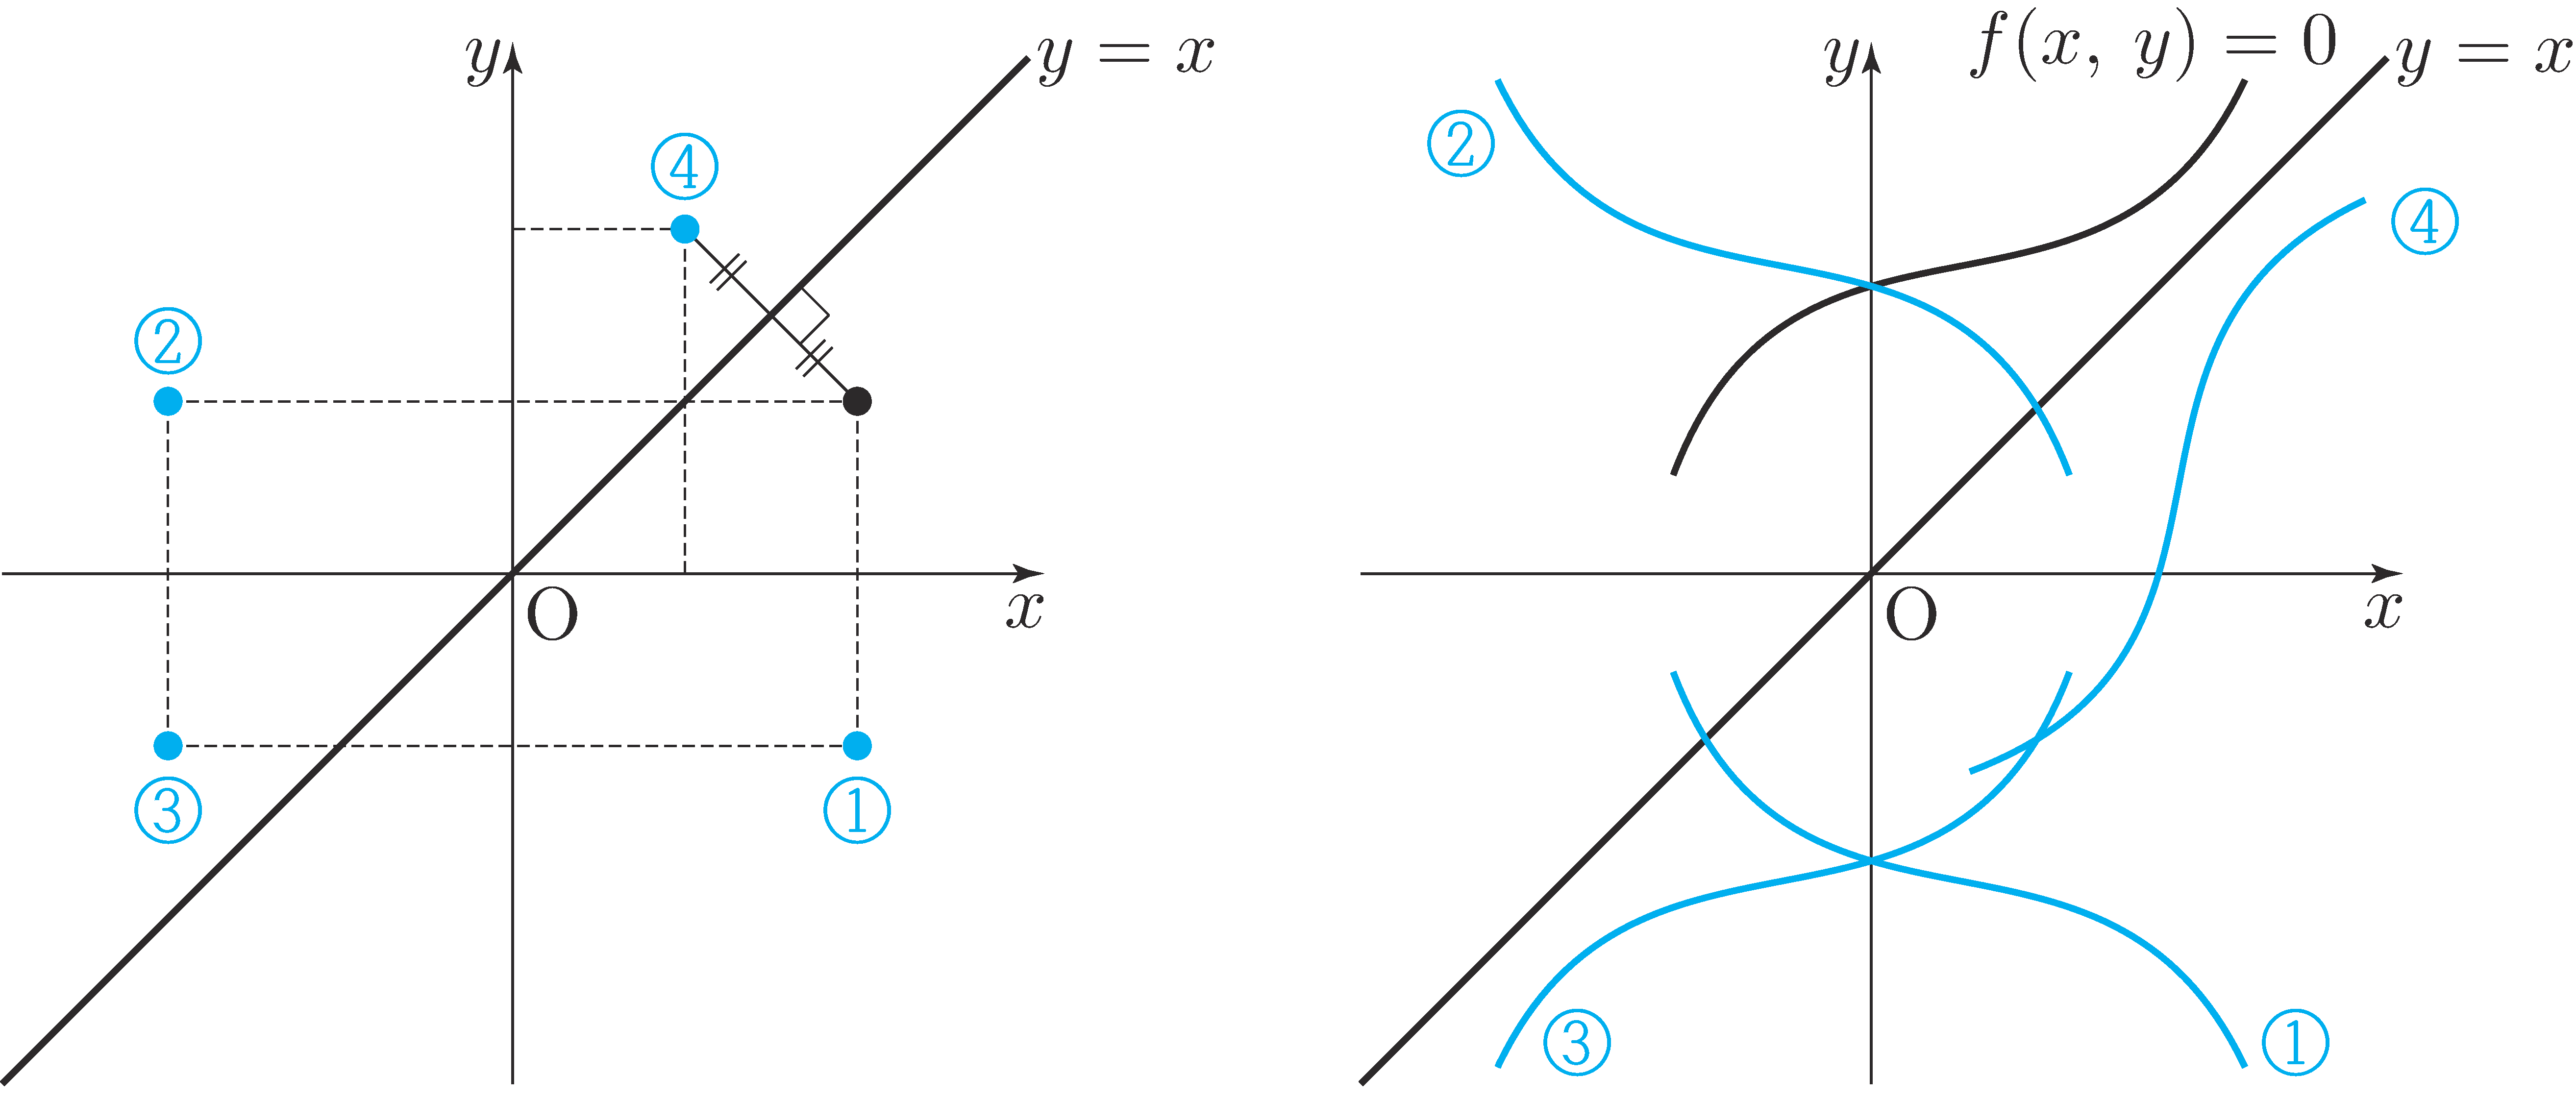
\includegraphics[scale=0.125]{pic0/pic150.pdf}
\end{center}좌표가 $\xy{x}{y}$인 점과 도형 $f(x,\:y)=0$을 $x$축, $y$축, 원점, 직선 $y=x$에 대하여 대칭이동한 점의 좌표와 도형의 방정식은 각각 다음과 같습니다.
\begin{justbox}
  \begin{enumerate}[label=\onum*]
    \item $x$축에 대하여 대칭이동 : $(x,\: -y)$, $f(x,\:-y)=0$
    \item $y$축에 대하여 대칭이동 : $(-x,\: y)$, $f(-x,\: y)=0$
    \item 원점에 대하여 대칭이동 :  $(-x,\: -y)$, $f(-x,\:-y)=0$
    \item 직선 $y=x$에 대하여 대칭이동 : $(y,\: x)$, $f(y,\: x)=0$
  \end{enumerate}
\end{justbox}

